\documentclass[../main.tex]{subfiles}
\graphicspath{{\subfix{..}}}

\begin{document}
\chapter{Reliability of machine learning methods}
\label{sec:janne}

\epigraph{``Psychohistory was the quintessence of sociology; it was the science of human behavior reduced to mathematical equations. The individual human being is unpredictable, but the reactions of human mobs, Seldon found, could be treated statistically''}{Isaac Asimov, Second Foundation}

\minitoc
%
% \textit{In this chapter I discuss the reliability of reconstruction algorithms, especially ML, in JUNO.}
%
% \textit{It is crucial for JUNO not only to reconstruct very precisely the energy of antineutrinos, but also to understand the quality of this reconstruction, and the differences in this between real data and the models assumed by the fits employed to perform the oscillation analysis.}
%
% \textit{We believe the first step in reliability studies is the comparison of the numerous reconstruction algorithms available in JUNO. In this goal, I present the implementation of a BDT for energy reconstruction that was developed by another scientist team in JUNO common software. I compare its resolution and behavior to OMILREC and use the combination method to probe for potential missing information in either of the algorithm}
%
% \textit{We also explore  the usage of an Adversarial Neural Network to produce perturbation in the event measurement (in recorded charge and time of PMT) that would distort the resulting energy spectrum while being invisible to the calibration.}
% \textit{I first discuss the method of this procedure, the Architecture that implement the method, the problematics and the implementation we present in this thesis. I finally present the training and the result obtained}
% \textit{We conclude this chapter by explaining that this first ANN prototype does not manage to generate perturbations that affect IBD events more than control sample events.  However, this exploration taught us several things, among which : it is very difficult to design an ANN able to introduce perturbations at the individual PMT level; some physics-informed guidance will be necessary to obtain an operational tool in the future.}
%
% \rule{\textwidth}{0.4pt}
As explained in previous chapters, JUNO is a precision experiment where the complete understanding of the effects at hand is crucial. As it will be illustrated in Chapter \ref{sec:joint_fit}, even small invisible biases or uncertainties could lead to the imposibility to run the measurements, or even worse, wrong NMO measurements. While the liquid scintillator technology is well known and straightforward, this is the first time it is deployed to such scale, and for such precision. This novelty bring its fair share of elements, effects or assumption, that, if they were to be overlooked, could cause issue.

We already shown a large variety of reconstruction algorithms, OMILREC for LPMT reconstruction in Section \ref{sec:juno:reco}, numerous machine learning algorithms in Section \ref{sec:juno:ml} and our own work in Chapters \ref{sec:jcnn} and \ref{sec:jgnn}. Those algorithms were compared to each others based on their performance as in \cite{qian_vertex_2021} but we are the first that looked into the correlation between the reconstruction. The combinations of algorithms shown in Section \ref{sec:jcnn:combination} show that some information elude the algorithms. To efficiently compare algorithms between each other, they need to be publicly available to the collaboration to studies their differences event by event.

To achieve this goal, I implemented a BDT for energy reconstruction, named BDTE which was developed by another research team, in the JUNO official software. The details of this implementation and its combination with OMILREC are presented in Section \ref{sec:janne:BDTE}.

Another way to ensure reliability is to challenge reconstruction algorithms with physically plausible perturbations in the PMT charge and time information.
The search for such effects could be done by hand, but the process would be tedious. We propose in this thesis a machine learning method to probe for those effects.  In Section \ref{sec:janne:method}, I describe the method behind the algorithm. In Section \ref{sec:janne:arch} I detail the architecture of our algorithm.
The training and the results of our method are presented in Section \ref{sec:janne:arch:training} . Finally, in section \ref{sec:janne:conclusion}, I conclude and discuss the prospects and possible improvements to bring to this work.


\section{BDT for energy reconstruction (BDTE)}
\label{sec:janne:BDTE}

To study the reliability of reconstruction algorithms it's necessary to be able to compare their reconstruction performance event by event. To ease the process, it is important that they are publicly available. JUNO's common software, discussed in Section \ref{sec:juno:software}, is based on the SNiPER framework \cite{lin_application_2017} which allows the packaging of the different steps of JUNO's analysis, from Monte Carlo (MC) data generation to event reconstruction, including the simulation of the PMTs' waveform reconstruction, electronic effects and the trigger system.

This framework is modular, with each module being a C++ class bound in Python. The execution of successive algorithms is orchestrated via Python scripts.


We could have implemented the algorithms presented in Chapters \ref{sec:jcnn} and \ref{sec:jgnn}, but since these are themselves not trivial, we chose to start with a simpler ML algorithm that presents similar energy reconstruction performances as OMILREC: a Boosted Decision Tree (BDT) for energy reconstruction developed by Gavrikov Arsenii et al. \cite{gavrikov_energy_2022}.
This BDT, named BDTE, is based on an aggregated feature approach where, from the set of $(Q, t)$ in LPMTs, a set of higher-order variables is computed and then fed to the BDT. The list of the aggregated features used by the BDT is presented in Table \ref{tab:janne:bdte:features}. These higher-order variables are extracted from the charge $Q$ and hit time $t$ distribution. It also depends on two straightforward interaction vertex estimators.


The first one is the charge barycenter
\begin{equation}
  \label{eq:janne:bdte:cc}
  \vec{r}_{cc} = \frac{\sum_i \vec{r}_{PMT,i} Q_i}{\sum_i Q_i}
\end{equation}
where $i$ index the fired PMT, $\vec{r}_{PMT, i}$ is the position vector of the $i$th PMT and $Q_i$ is the charge it collected.

The second estimator is the hit time barycenter
\begin{equation}
  \label{eq:janne:bdt:cht}
  \vec{r}_{ht} = \frac{1}{\sum_i \frac{1}{t_i + c}} \sum_i \frac{\vec{r}_{PMT, i}}{t_i + c}
\end{equation}
where $t_i$ is the time of collection of the $i$th PMT and $c = 50$ ns a constant to prevent divergence when $t_i$ is 0.

\begin{table}[ht]
  \centering
  \begin{tabular}{|l | l|}
    \hline
    Feature & Description \\
    \hline
    AccumCharge             & Sum of the charge collected by every LPMT \\
    $R_{ht}               $ & Radius reconstructed by the hit time barycenter  \\
    $z_{cc}               $ & $z$ component of the vertex reconstructed by the charge barycenter \\
    $\sigma \text{PE}     $ & Standard deviation of the distribution of collected PE per PMTs \\
    $N_{PMT}              $ & Number of fired PMTs \\
    $\text{ht}_{Kurtosis} $ & Kurtosis of the hit time distribution \\
    $\text{ht}_{25\%-20\%}$ & Difference between the 25\% and 20\% percentiles of the hit time distribution \\
    $R_{cc}               $ & Radius reconstructed by the center of charge barycenter \\
    $\text{ht}_{5\%-2\%}  $ & Difference between the 5\% and 2\% percentiles of the hit time distribution \\
    $\langle \text{PE} \rangle$ & Mean number of PE collected per PMTs \\
    ${\cal J}_{ht}        $ & Jacobian of the hit time distrbution \\
    $\phi_{cc}            $ & $\phi$ component in spherical coordinate of the charge barycenter \\
    $\text{ht}_{35\%-30\%}$ & Difference between the 25\% and 20\% percentiles of the hit time distribution \\
    $\text{ht}_{20\%-15\%}$ & Difference between the 20\% and 15\% percentiles of the hit time distribution \\
    $\text{PE}_{35\%}     $ & Value of the 35\% percentile of the charge distribution \\
    $\text{ht}_{30\%-25\%}$ & Difference between the 30\% and 25\% percentiles of the hit time distribution \\
    \hline
  \end{tabular}
  \caption{Summary of the aggregated features used by the BDT to reconstruct the IBD energy. The charge barycenter and hit time barycenter vertex estimators are detailed in Eq. \ref{eq:janne:bdte:cc} and \ref{eq:janne:bdt:cht} respectively}
  \label{tab:janne:bdte:features}
\end{table}

The performance of this BDT, as published by Gavrikov Arsenii et. al, is reported in Figure \ref{fig:janne:bdte:orignal_perf}. This BDT was originally developed in Python and consisted of a collection of Python scripts for the training and the evaluation.

As stated before, JUNO software is composed of C++ modules orchestrated through Python scripts. The technical challenge was to extract the data from the internal representation of the event in JUNO software, the Event Data Model (EDM), into a comprehensible format for Python. This task, which was previously done via data pre-processing by Python scripts, had to be internalized within the software. The computation of the aggregated features was migrated from the Python scripts into C++ modules. The final step was to fetch the reconstruction results of the algorithm into the C++ framework to save the results in the EDM.

We validated that the aggregated features were consistent between the original version and the implementation in JUNO software. With the help of Arsenii, we were able to compare over 1000 events, and for the majority of the features, the relative difference between his and ours was either 0 or on the order of $10^{-15}$, with the exception of three features: $R_{cc}$, $R_{ht}$, and $z_{cc}$. For these three features, the relative difference is about $10^{-6}$, which, while small, is still surprisingly high for numerical computation. The distributions of the relative differences for these features are presented in Figure \ref{fig:janne:feat_diff}.

We investigated the source of those discrepancies. The difference in computation environments, Python using the Numpy \cite{harris_array_2020} and C++ using the standard library in our cases, is most probably the source. As they are coming from the computation of the barycenter in Eq. \ref{eq:janne:bdte:cc} and \ref{eq:janne:bdt:cht}, it could come from differences in the compiling optimization in the weighted sum. We consider that those difference are still small so that the performance of the BDT are unaffected.

We investigated the source of these discrepancies. The difference in computation environments—Python using Numpy \cite{harris_array_2020} and C++ using the standard library in our case—is most likely the cause. Since the discrepancies arise from the computation of the barycenter in Eq. \ref{eq:janne:bdte:cc} and \ref{eq:janne:bdt:cht}, they may result from differences in compiler optimization during the weighted sum calculation. We consider that these differences are still small enough that the performance of the BDT is unaffected.


\begin{figure}[ht]
  \centering
  \begin{subfigure}[t]{0.32\linewidth}
    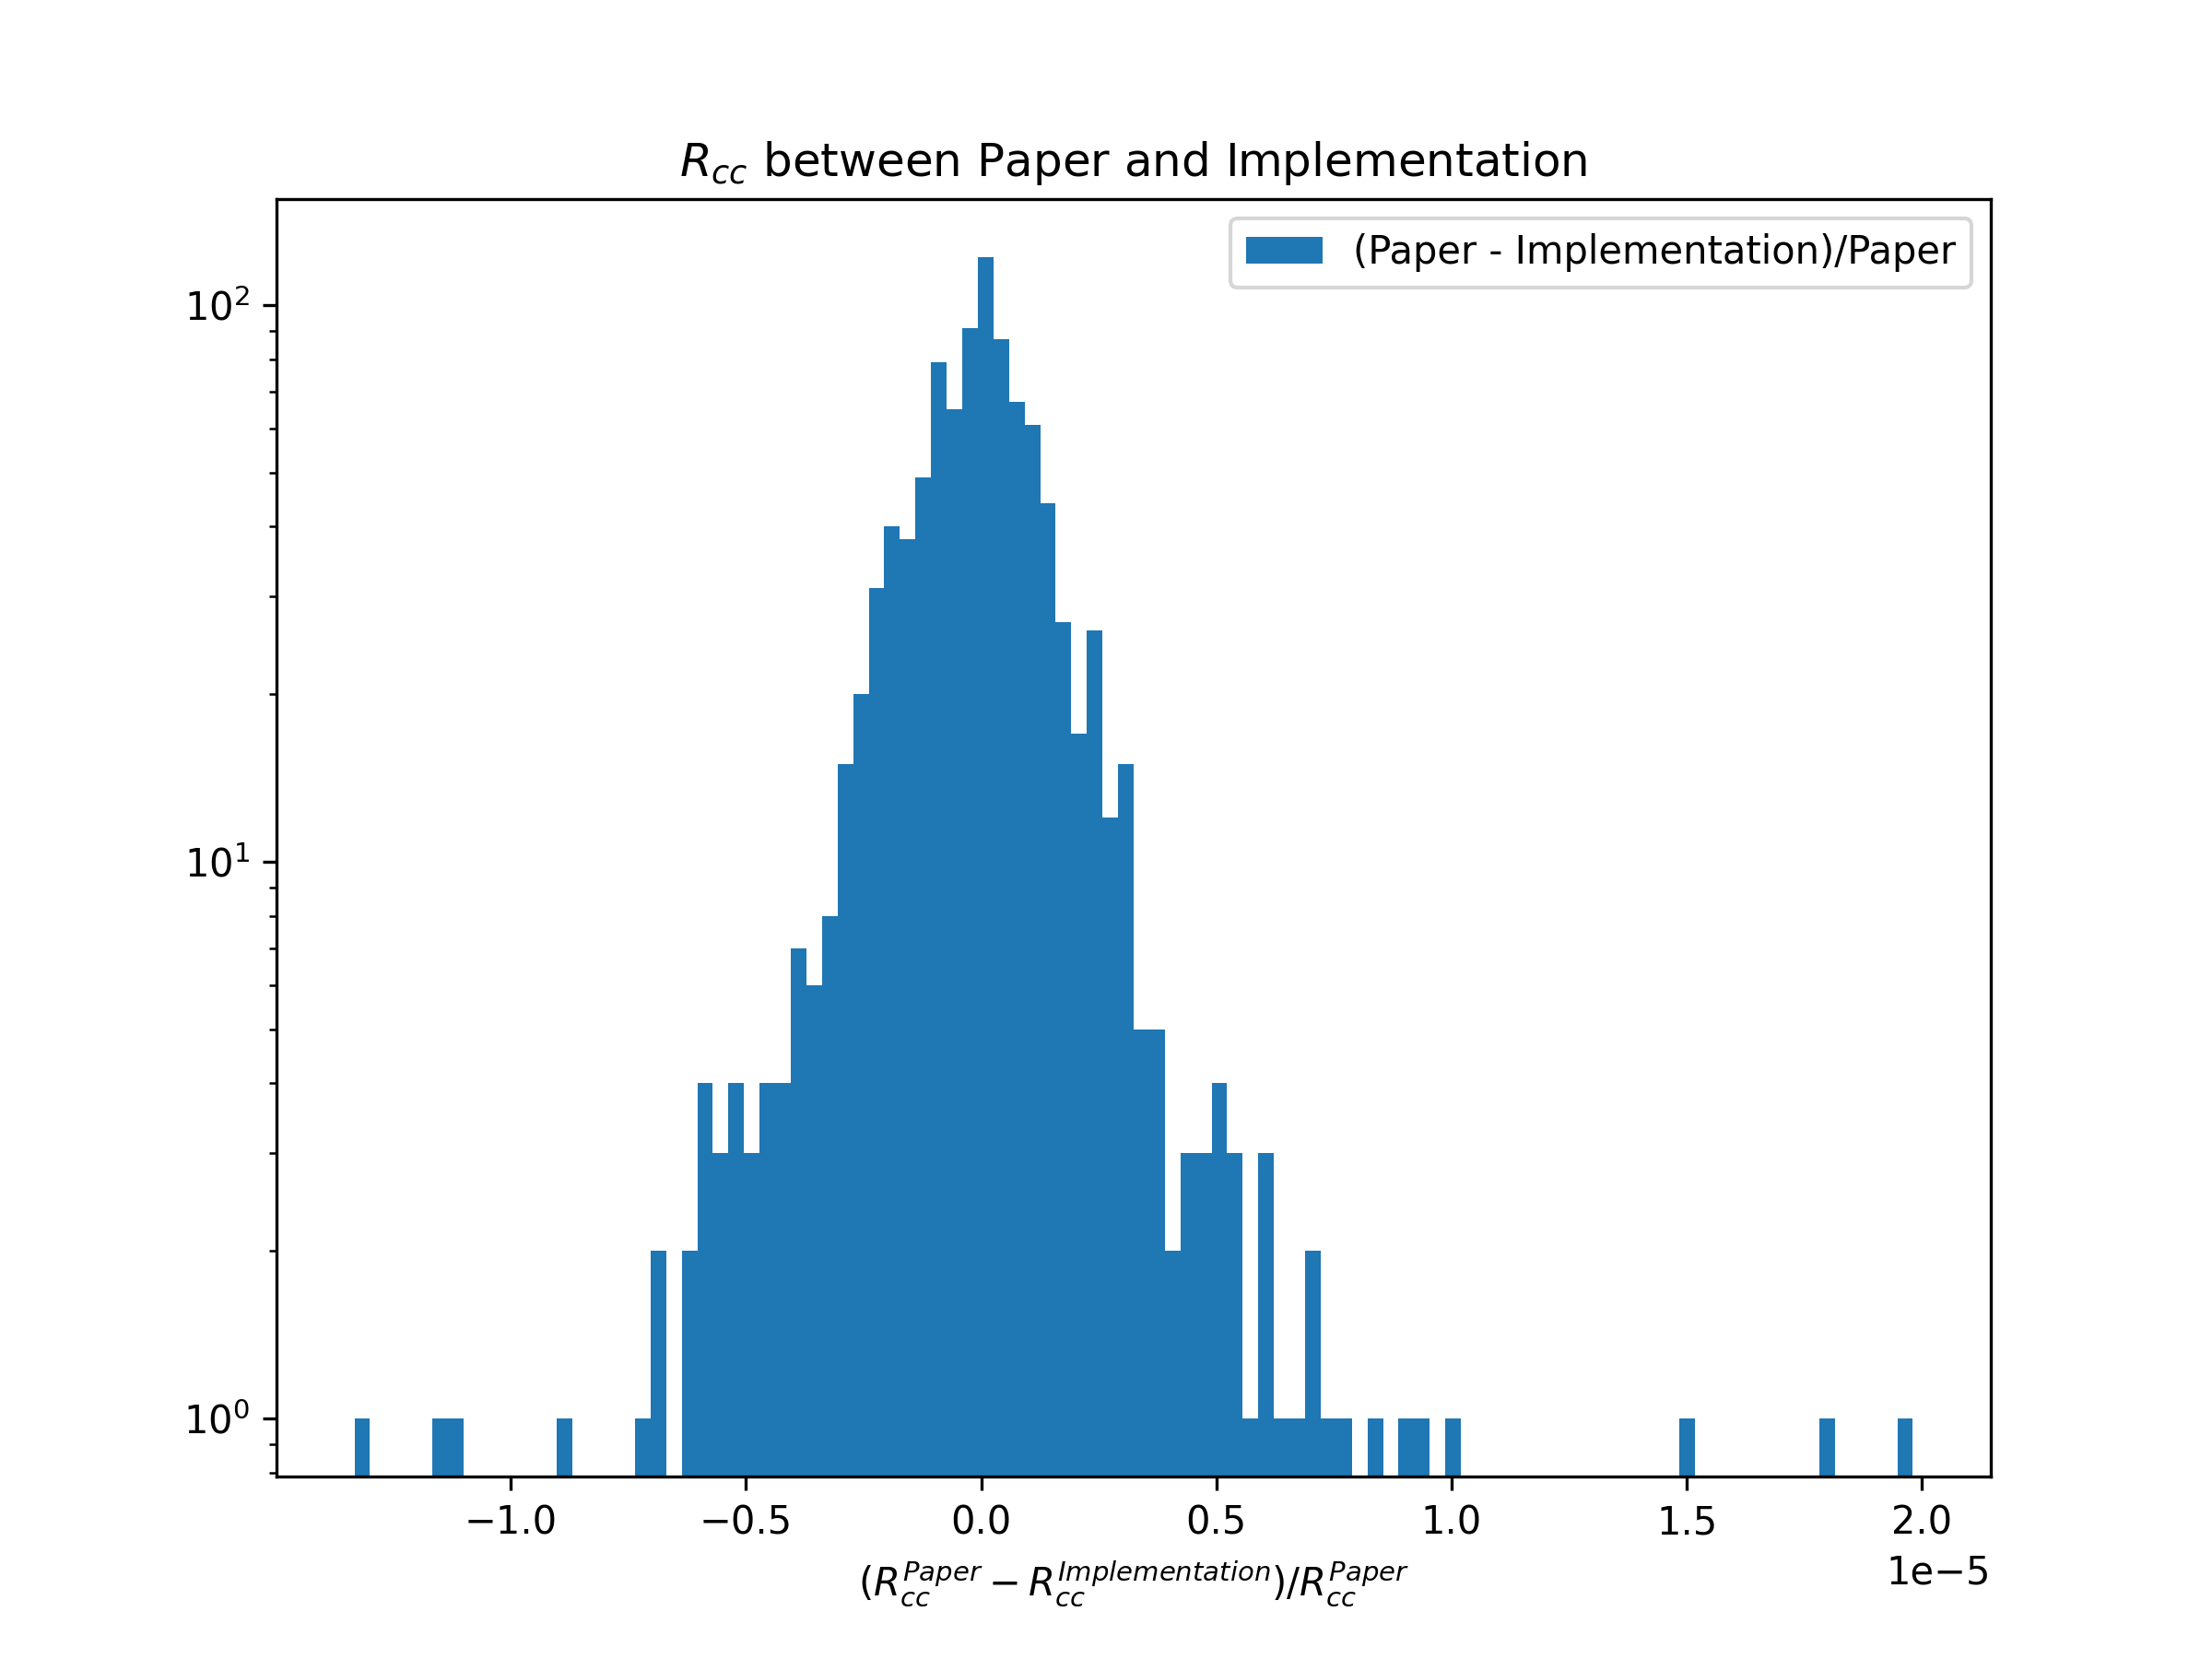
\includegraphics[width=\linewidth]{images/janne/bdte/R_cc_diff.png}
  \end{subfigure}
  \hfill
  \begin{subfigure}[t]{0.32\linewidth}
    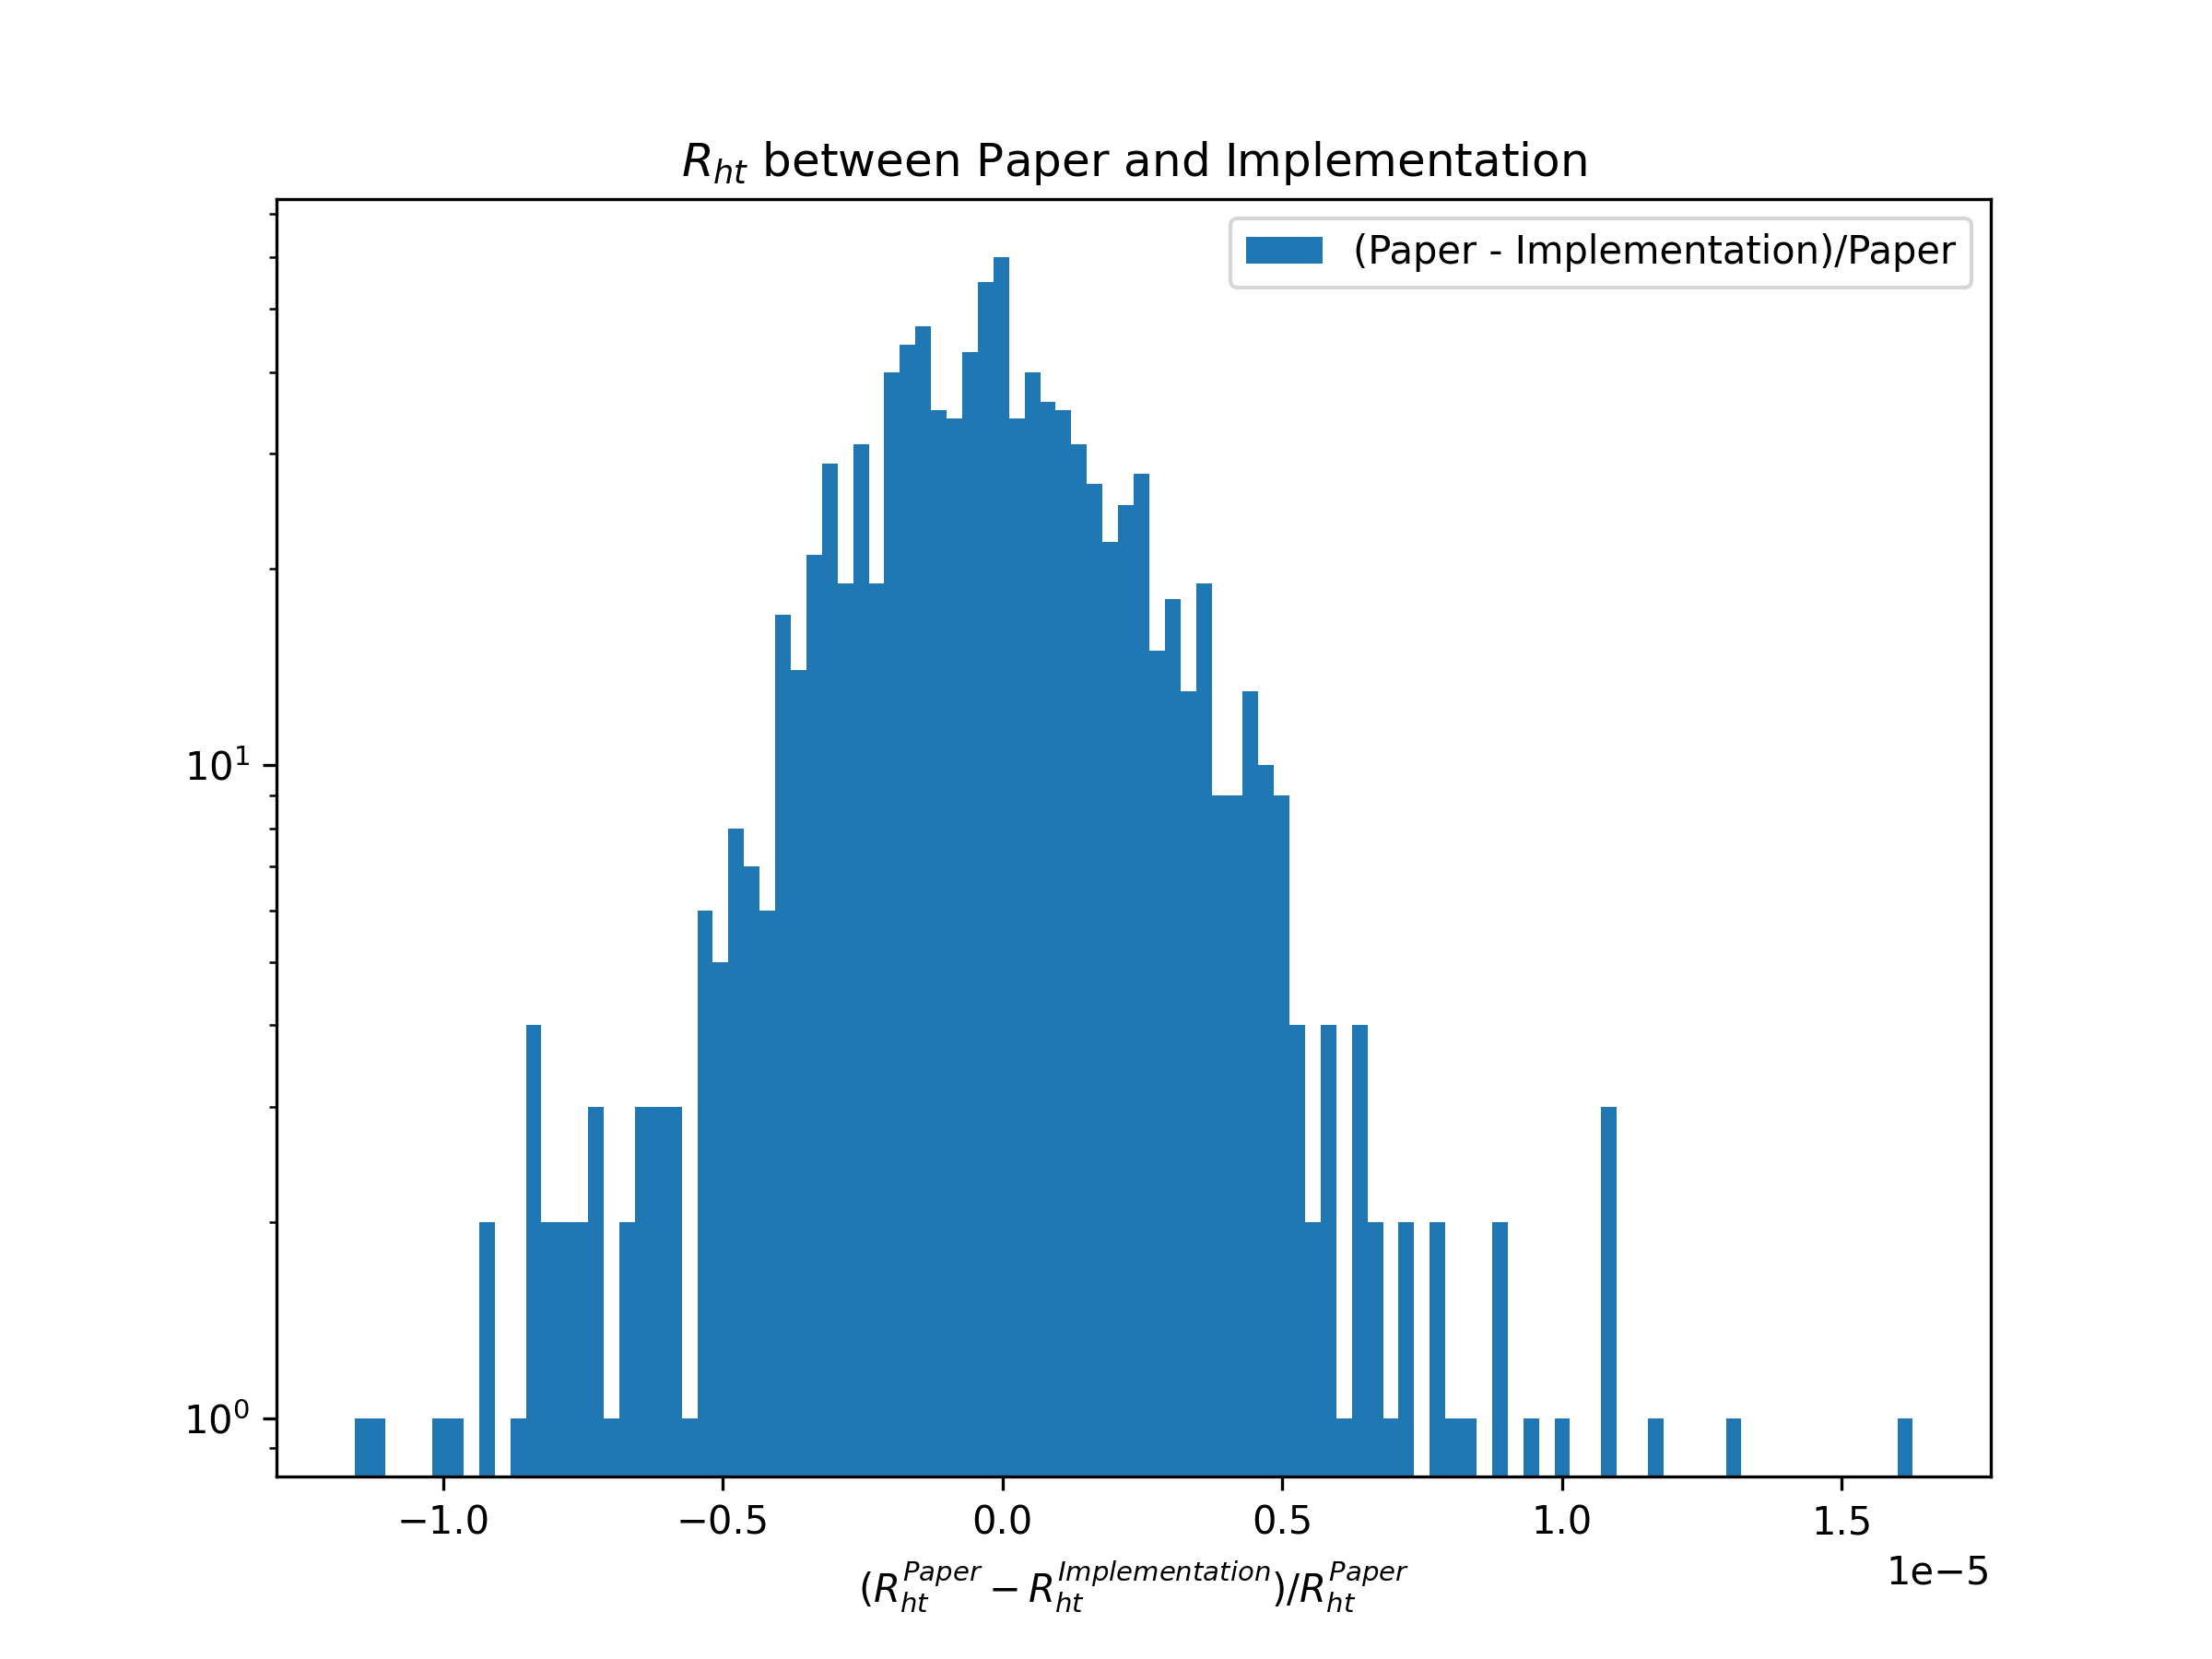
\includegraphics[width=\linewidth]{images/janne/bdte/R_cht_diff.png}
  \end{subfigure}
  \hfill
  \begin{subfigure}[t]{0.32\linewidth}
    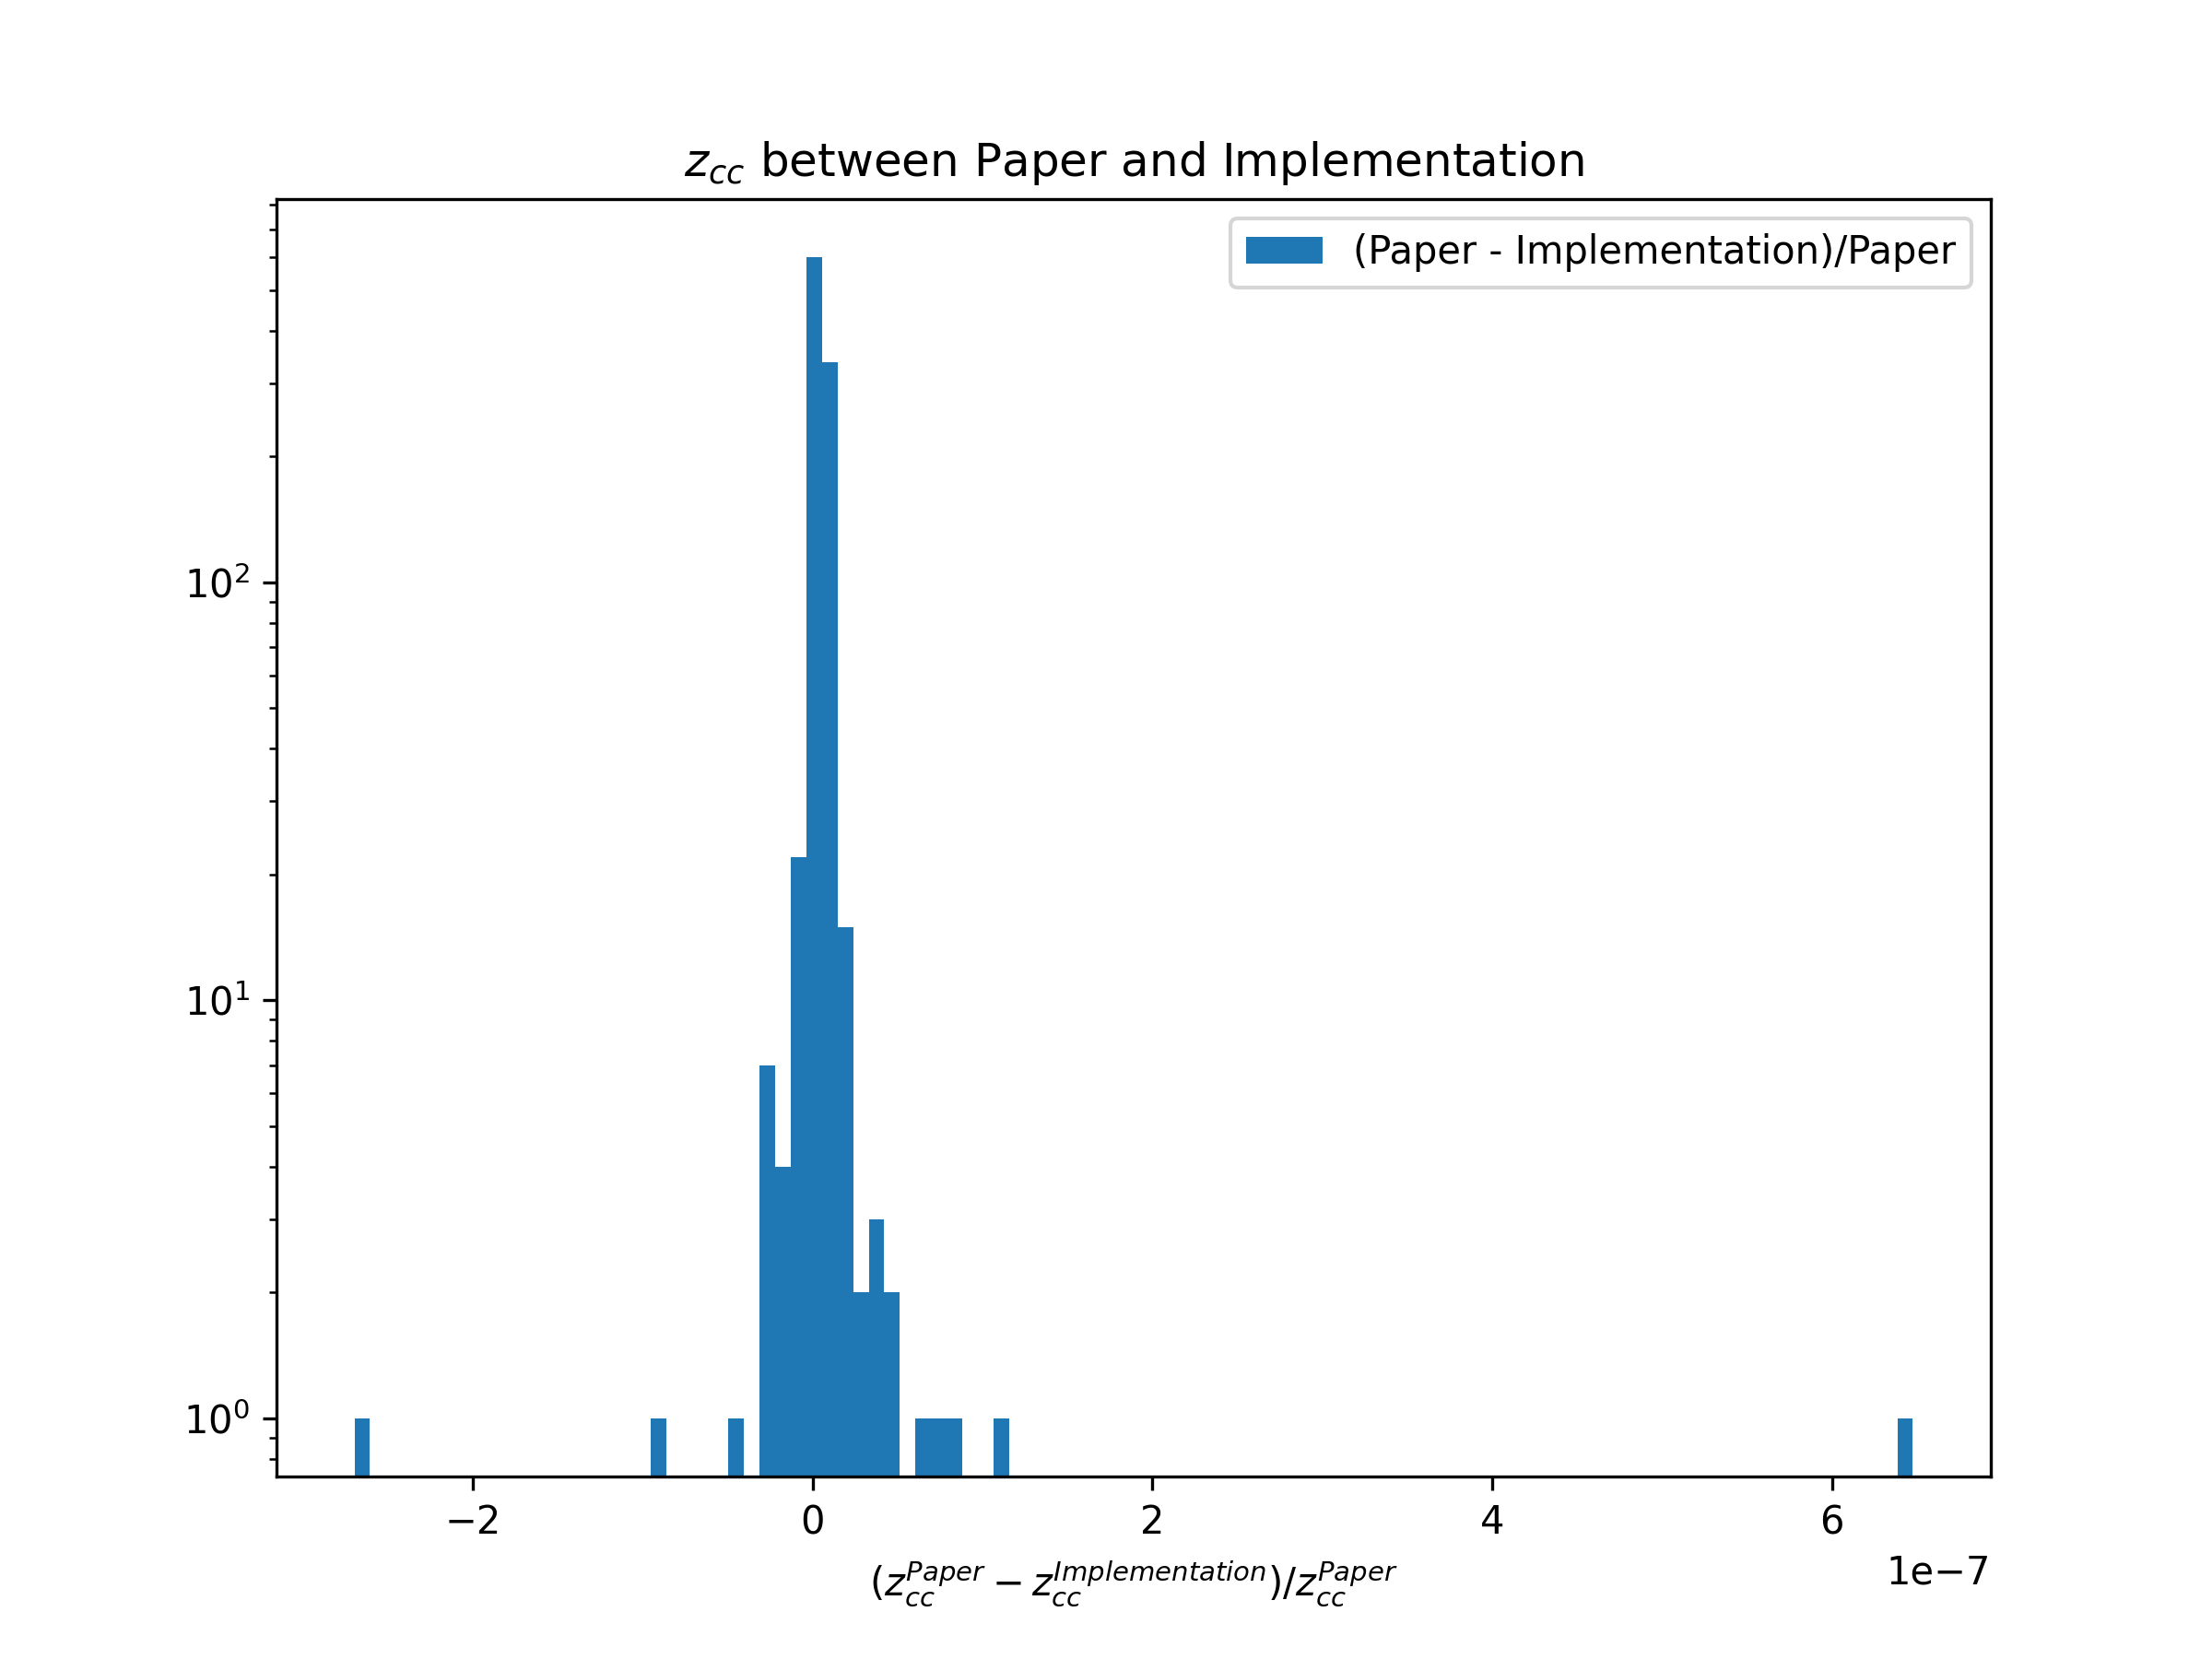
\includegraphics[width=\linewidth]{images/janne/bdte/z_cc_diff.png}
  \end{subfigure}
  \caption{Relative difference between the features computed by Gavrikov et. al (superscripted Paper) and our implementation (superscripted Implementation)}
  \label{fig:janne:feat_diff}
\end{figure}

The performance of our implementation of BDTE compared to the results presented in \cite{gavrikov_energy_2022} are presented in figure \ref{fig:janne:bdte:implementation_perf}. The performance are compatibles.

\begin{figure}[ht]
  \centering
  \begin{subfigure}[t]{0.58\linewidth}
    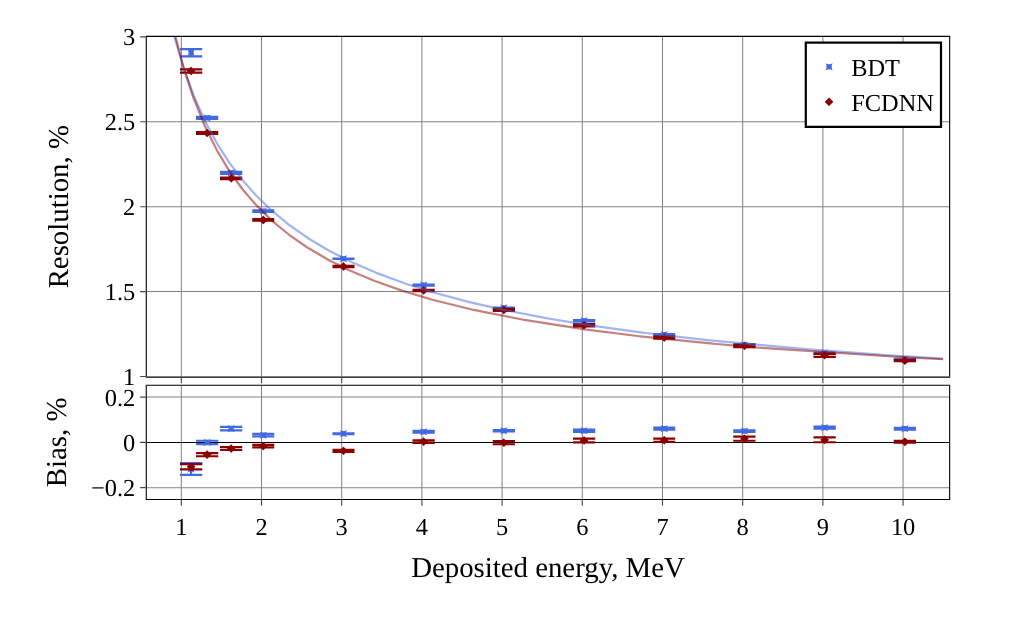
\includegraphics[width=\linewidth]{images/janne/bdte/bdte_perf.png}
    \caption{}
    \label{fig:janne:bdte:orignal_perf}
  \end{subfigure}
  \hfill
  \begin{subfigure}[t]{0.38\linewidth}
    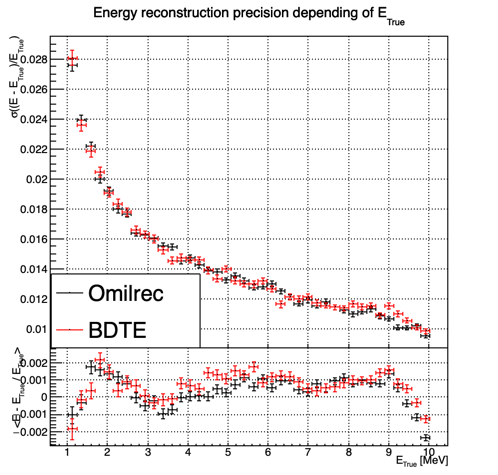
\includegraphics[width=\linewidth]{images/janne/bdte/e_rec_vs_e_true.png}
    \caption{}
    \label{fig:janne:bdte:implementation_perf}
  \end{subfigure}
  \caption{Resolution of BDTE \textbf{On the left: } as reported by Gavrikov Arsenii et. al in \cite{gavrikov_energy_2022}, \textbf{On the right: } once implemented in JUNO common software. On the right plot is also reported the reconstruction performance of the OMILREC algorithm. The OMILREC algorithm $E_{vis}$ has been corrected to $E_{dep}$ following the procedure detailled in Annex \ref{sec:annex:evis}.}
  \label{fig:janne:bdte:perf}
\end{figure}

The reconstruction using BDTE was implemented in JUNO's common software but Gavrikov et al. also detail the training and hyper-optimization. JUNO Monte Carlo is likely to evolve during the construction phase and will be further adjusted using calibration. The implementation of those procedures, the training and optimization, will be required as BDTE re-training and re-optimisation will be required with each JUNO software update.

Figure \ref{fig:janne:bdte:implementation_perf} shows that the resolution of BDTE is very close to OMILREC. We measured the correlation between their errors:
\begin{equation}
  \label{eq:janne:bdte:corr}
\mathrm{Corr}(E_{BDTE} - E_{dep}, E_{OMILREC} - E_{dep})
\end{equation}

If the correlation is small enough, it hints at possible improvements in the IBD reconstruction. The correlation between errors for different energy and event radius in the detector is presented in Figure \ref{fig:janne:bdte:corr}. We see that for the vast majority of the $(R^3, E)$ phase space, the correlation is > 0.995, down to $\sim$ 0.98 in the $R \approx 9$ m and $R > 17$ m regions. Such high correlations indicate that there is close to no improvement that can be found in these algorithms.

\begin{figure}
  \centering
  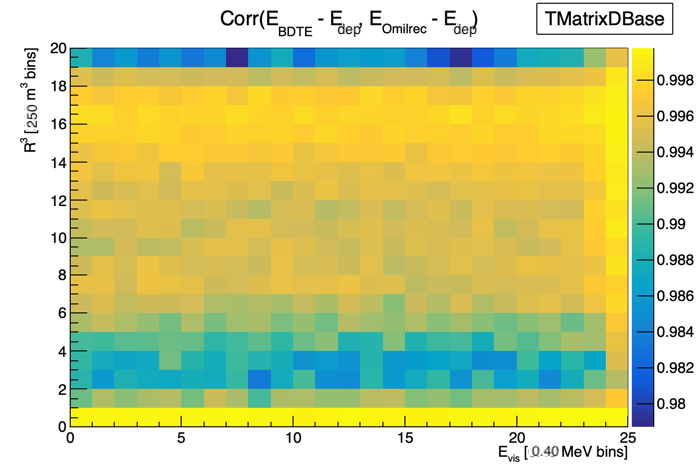
\includegraphics[height=7cm]{images/janne/bdte/corr_bdte_omilrec.png}
  \caption{Correlation between the errors in energy reconstruction between BDTE and OMILREC (Eq. \ref{eq:janne:bdte:corr}). The correlation is computed in $R^3$ bins of 216 m$^3$ between 0 and 5000 m$^3$, 0 and 17 m in y axis, and in 0.40 MeV bins between 1.022 and 10.022 MeV of deposited energy.}
  \label{fig:janne:bdte:corr}
\end{figure}



\section{Adversarial method}
\label{sec:janne:method}
%\begin{itemize}
%  \item JUNO needs very good understanding of reconstruction
%  \item Estimator combination shows that there can be improvement due to simplfication and that NN/reco methods can have hard time grasping all the detector effect.
%  \item If there is potential failure point, we need to search for them
%  \item La mesure de la NMO est tres sensible (see $alpha_{qnl}$ joint fit chapter)
%\end{itemize}

As introduced at the beginning of the chapter, JUNO needs a very good understanding of the biases and effects affecting its reconstruction, as a small bias could distort the mass ordering measurement. To calibrate those biases and effects, JUNO relies on multiple sources that can be located at various points in the detector. The calibration strategy is already discussed in Section \ref{sec:juno:calib} and shows calibration sources of gammas, neutrons, and positrons (Table \ref{tab:juno:calib_source}), with the catch that the positrons will annihilate inside the encapsulation and only the two 511 keV gammas will deposit energy in the LS.

None of the calibration sources considered are positron events. While electrons and positron events should be pretty similar in their interaction with the electronic cloud of the LS atoms, electron events are missing the two annihilation $\gamma$ photons and the potential of forming a positronium \cite{schwarz_measurements_2018}. The topology of the event is localized in a region of the order of magnitude of our reconstruction performance. A few nanoseconds between the energy deposition and the positronium annihilation against a time transit spread between 3 and 6 ns, depending on the PMT type \cite{rodphai_20-inch_2021, liao_study_2017, li_characterization_2018}. The $\gamma$ from the positron annihilation will travel distances of the order of magnitude of the typical LPMT resolution of 8 cm (see Section \ref{sec:juno:reco}).

Another natural calibration source is the $^{12}B$ spectrum. The $^{12}B$ is a cosmogenically produced isotope through the passage of muons inside the LS. The $^{12}B$ decays via $\beta^-$ emissions with a Q value of 13.5 MeV, with more than 98\% of the decay resulting in ground state $^{12}C$. The $^{12}B$ events will be cleanly identified by looking for delayed high-energy $\beta$ events after an energetic muon. Due to its natural causes, the $^{12}B$ events will be uniformly distributed in the detector. The calibration strategy consists of fitting the energy spectrum of $^{12}B$ with the results of the simulation to adjust the simulation parameters. Both sources will be used to \textit{control} the response of the detector.

Unlike lasers and radioactive sources, from which the localization and energy will be well known, the individual events of $^{12}B$ will be unknown, with only the localization loosely constrained by the muon track. Only higher-order observables such as the energy distribution will be accessible.

All of those considerations could hide potential unknown or undetected effects that could lead to issues in the mass ordering analysis. But, while we have an idea of where the issues could come from, the manual production of event perturbations that go unseen in the calibration would be tedious. That's why we propose to use an Adversarial Neural Network (ANN) to produce those perturbations if they exist. A schematic of the concept is presented in Figure \ref{fig:janne:method:schema}.

\begin{figure}[ht]
  \centering
  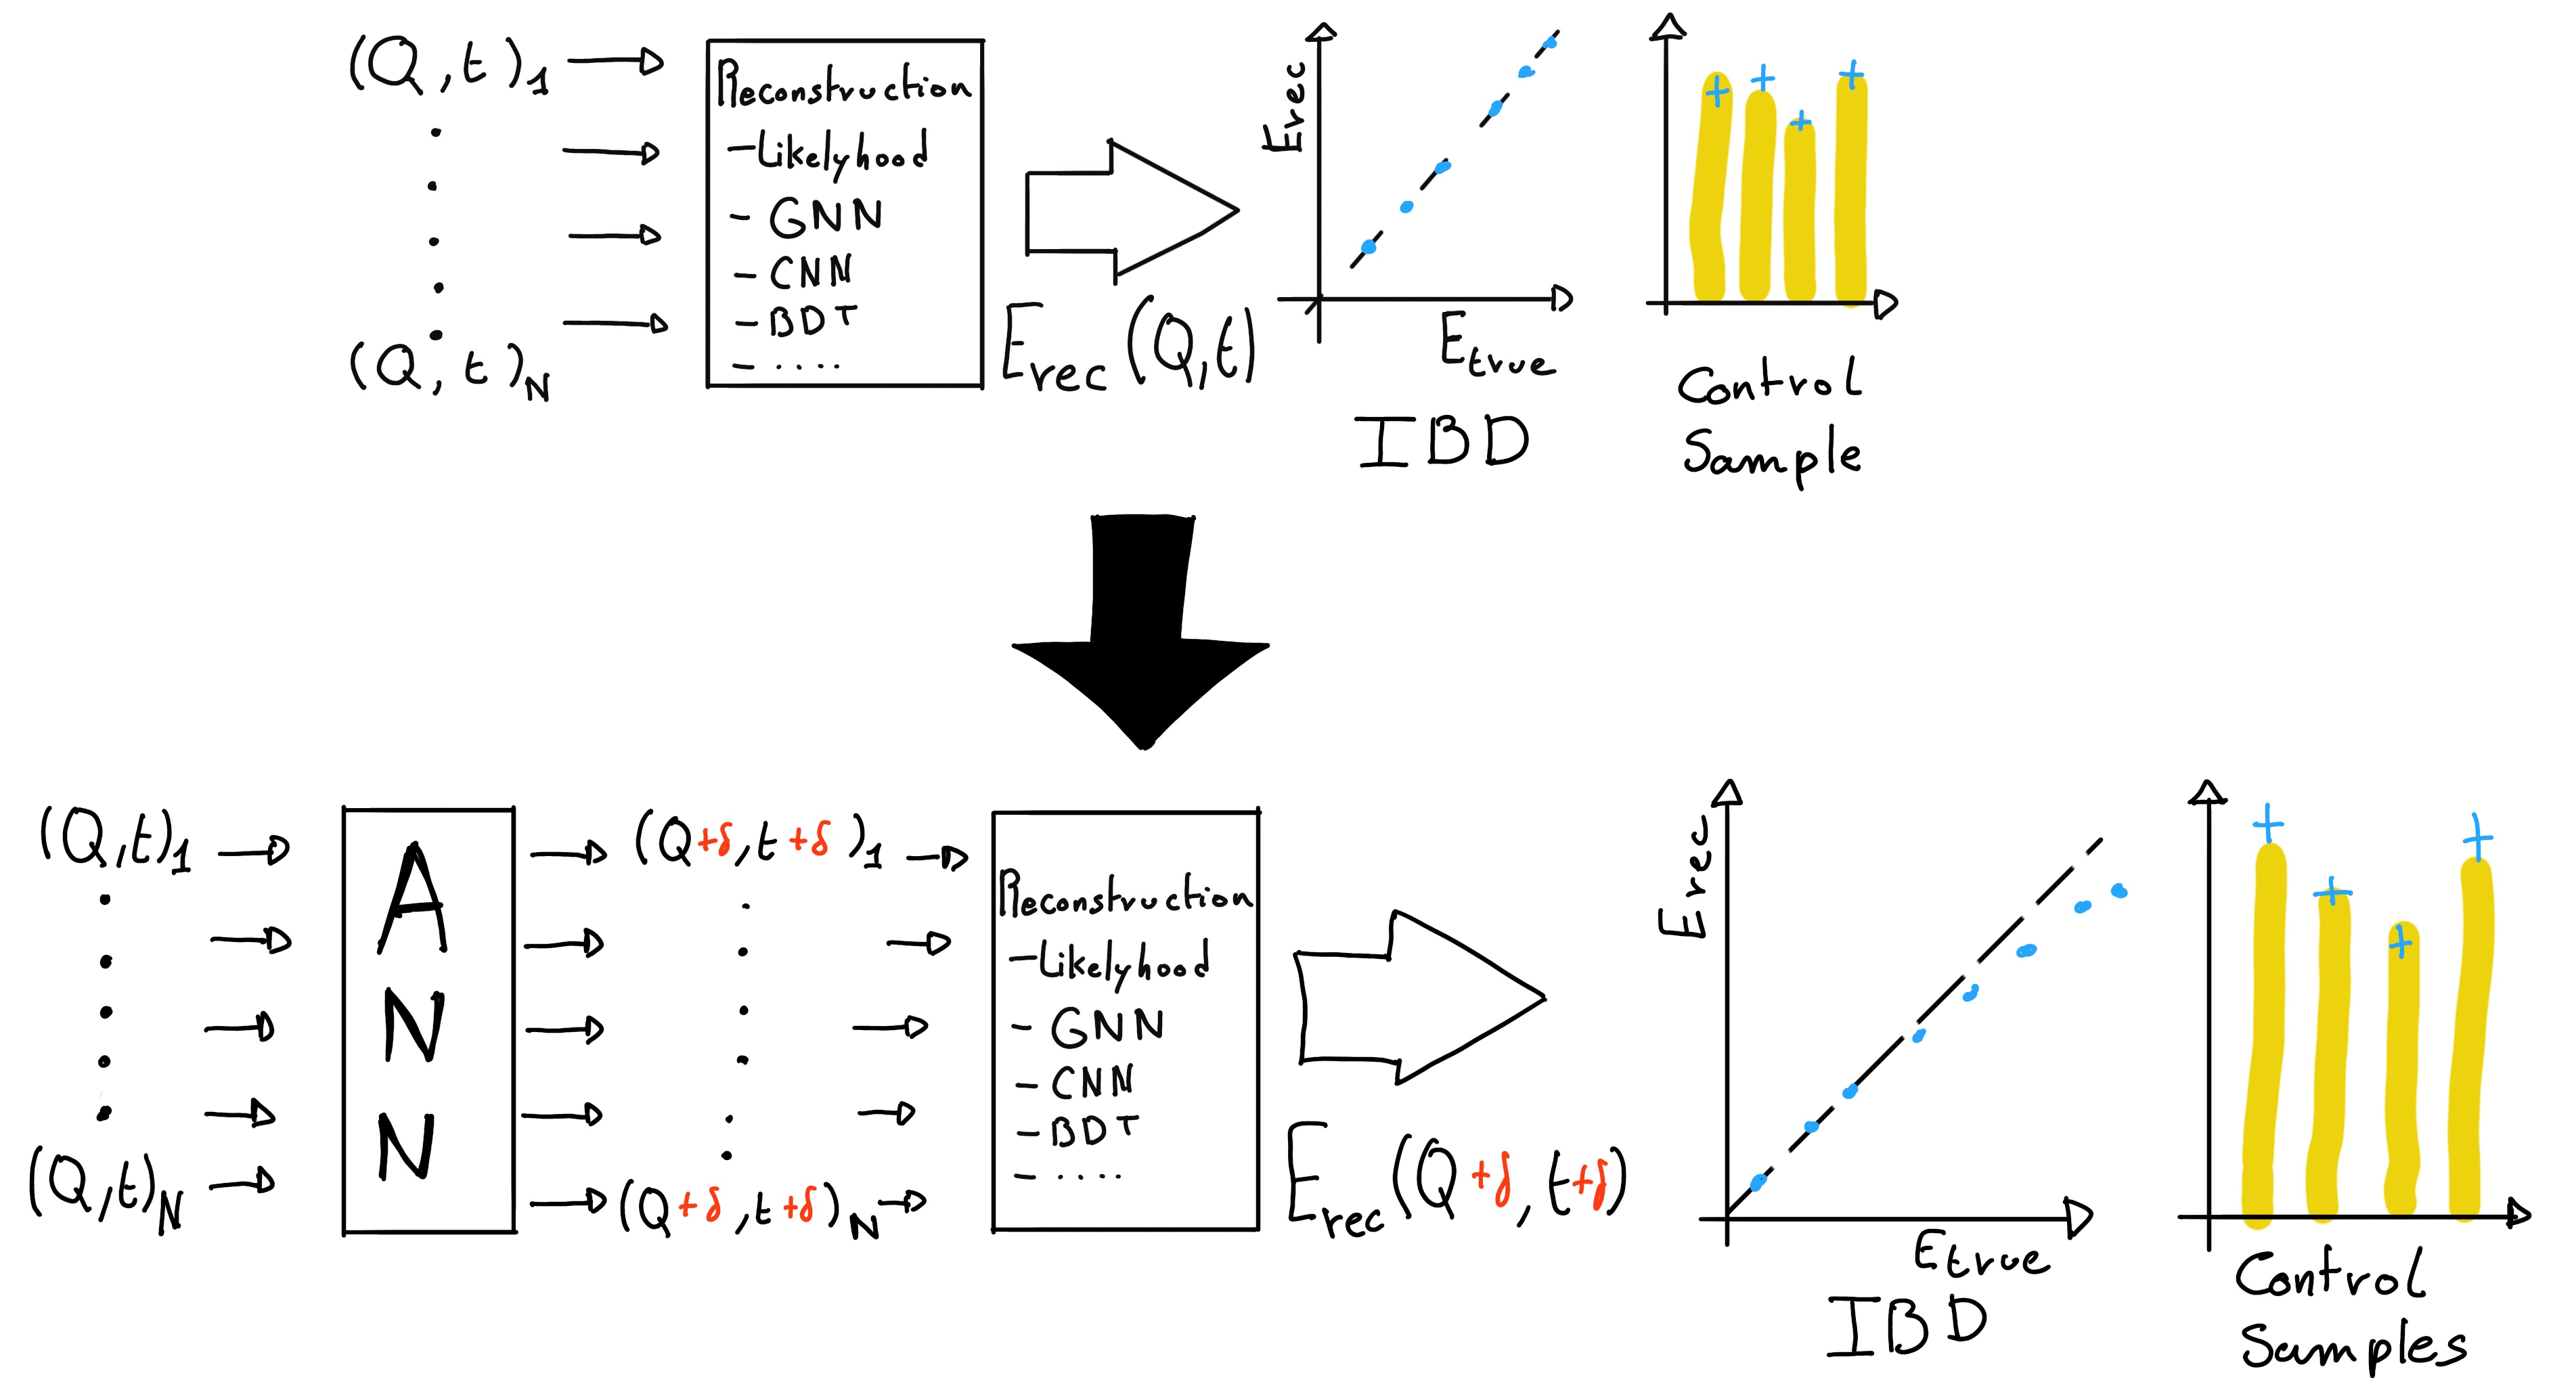
\includegraphics[width=\linewidth]{images/janne/ann_method.jpg}
  \caption{Schema of the method to discover vulnerabilities in the reconstruction methods. \textbf{On the top} of the image, the standard data flow. The individual charge and times are fed to a reconstruction algorithm. From the reconstructed energies, we can produce an IBD spectrum and compute control observables from the control samples. \textbf{On the bottom}, the same data flow but we add an ANN between the input and the reconstruction. The ANN will slightly change the input charge and time so the reconstruction algorithm inaccurately reconstruct the IBD energy, but the perturbation is not visible in the control samples.}
  \label{fig:janne:method:schema}
\end{figure}

This network should produce physically plausible perturbations that would not be seen by the calibration system but also by the visualization of the event. If the ANN manages to produce such perturbations, we can derive systematic uncertainties from it. If it fails to find any, it is a proof of robustness for the targeted reconstruction method.

For this study, we consider a ``physics'' dataset composed of 1M positron events from J23, uniformly distributed in the Central Detector (CD) and in deposited energy between $E_{dep} \in [1.022; 10.022]$. This set represents the IBD events we want to the reconstruction to be fooled on.

We use a second “control” dataset of 1M electron events from J23, also uniformly distributed in the detector and over the same energy range. They mimic the energy deposition of $^{12}B$ decay and are used as the sample to compute the control observables.



\section{ANN Architecture}
\label{sec:janne:arch}
%\begin{itemize}
%  \item Expliquer la problematique dans l'architecture
%  \item Ambition de pouvoir etre appliqué a toutes les methodes, pas que NN
%  \item Pb techique: descente de gradient
%  \item Présenter la loss
%\end{itemize}
We can describe the goal of the ANN by using following loss function:
\begin{equation}
  \label{eq:janne:loss}
  \mathcal{L} = \mathcal{L}_{adv} + \mathcal{L}_{reg}
\end{equation}
where $\mathcal{L}_{adv}$ is the adversarial loss, which is minimal when the reconstruction is ``broken''. We thus need to define what is a \textit{wrong} reconstruction. We choose to define it through the correlation between the reconstructed and deposited energy
\begin{equation}
  \label{eq:janne:ladv}
  \mathcal{L}_{adv} = |\mathrm{Corr}(E'_{rec}, E_{rec})|
\end{equation}
where $E'_{rec}$ and $E_{rec}$ are the reconstructed energies after and before perturbation respectively.
This loss is positive or null and is minimal when the reconstructed energy after perturbation is decorrelated with the original reconstruction.

The term $\mathcal{L}_{reg}$ is the regularisation term, which is minimal when the control variables are correctly reconstructed
\begin{equation}
  \mathcal{L}_{reg} = \sum_\lambda (O^{rec}_\lambda - O^{th}_\lambda)^2
\end{equation}
where $\lambda$ index the different control observables that will be considered in this study. It's minimal when the control observables after perturbation $O^{rec}_\lambda$ are coherent with their expected values $O^{th}_\lambda$.
In this exploratory work, we choose as the control observable the difference between the reconstructed position and energy and the ground truth from the Monte Carlo simulation
\begin{equation}
  \label{eq:janne:lreg}
  \mathcal{L}_{reg} = \sum_{\lambda \in \{x, y, z, E\}} (\lambda_{rec} - \lambda_{true})^2
\end{equation}

To these two loss, we adjoin a penalty term $P$
\begin{equation}
  {\cal L} = {\cal L}_{adv} + {\cal L}_{reg} + P
\end{equation}
This penalty $P$ is here to prevent the ANN from producing event too different from the initial event. It will be further detailed in Section \ref{sec:janne:arch:ann}.

We see that the final loss is an equilibrium between the adversarial and regularisation loss.

\subsection{Back-propagation problematic}
\label{sec:janne:back_prop}

We would like this method to be applicable to any kind of reconstruction algorithm but this complicated considering standard training method through backward-propagation, discussed in details in Section \ref{sec:ml:optim}. For explanation, let's define the application of the reconstruction algorithm as $\mathcal{F}$ on an event $X$, resulting in the prediction $Y$, and the application of the ANN $\mathcal{G}$ on $X$ to give a perturbed event $X'$. We can parametrize the equation \ref{eq:janne:loss}
\begin{align}
  Y = \mathcal{F}(X); ~~& Y' = \mathcal{F}(X') = \mathcal{F}(\mathcal{G}(X))
\end{align}
\begin{equation}
  \mathcal{L} \equiv \mathcal{L}(\mathcal{F}(\mathcal{G}(X)), Y_t)
\end{equation}
where $Y_t$ is the reconstruction target of $Y$.

Now if we consider the parameters $\bm{\theta}$ of the ANN on which we want to optimize $\mathcal{L}$, in the backward-propagation optimisation framework we need to compute
\begin{equation}
  \frac{\partial \mathcal{L}(\mathcal{F}(\mathcal{G}(X)))}{\partial \bm{\theta}}
\end{equation}
which, when using the chain rule, become
\begin{equation}
  \frac{\partial \mathcal{L}(\mathcal{F}(\mathcal{G}(X)))}{\partial \bm{\theta}} = \frac{\partial \mathcal{G}}{\partial \bm{\theta}} \cdot \frac{\partial \mathcal{F}}{\partial \mathcal{G}} \cdot \frac{\partial \mathcal{L}}{\partial \mathcal{F}}
\end{equation}

The terms $\frac{\partial \mathcal{G}}{\partial \bm{\theta}}$ and $\frac{\partial \mathcal{L}}{\partial \mathcal{F}}$ are easily computable but $\frac{\partial \mathcal{F}}{\partial \mathcal{G}}$ depends on the nature of the reconstruction algorithm.


While it comes naturally when using neural network algorithms, it's not so trivial for other types of algorithms like likelihood. Solutions exist to optimize networks that work in complex, non-differentiable environments, such as \textit{Deep Reinforcement Learning} \cite{kiran_deep_2021, vinyals_grandmaster_2019}, but as a first prototype, we will restrict ourselves to neural networks for the reconstruction algorithm.

The choice to use gradient descent, and therefore neural networks, also allowed us to keep all technical software development wrapped in the same language and framework, PyTorch \cite{ansel_pytorch_2024}.

The backward-propagation introduce a second issue. At the beginning of the subsection we introduce $X' = \mathcal{G}(X)$, the event after perturbation. It's an input of the reconstruction $\mathcal{F}$, thus, let's say that the event, in its form $X$, is a list of tuples $(id, Q, t)$ which are the hit on the PMT $id$. If $\mathcal{F}$ require the information to be formatted in a specific way (graph, images, ...) via an algorithm $\tau(X)$, it means that
\begin{equation}
  \frac{\partial \mathcal{L}(\mathcal{F}(\tau(\mathcal{G}(X))))}{\partial \bm{\theta}} = \frac{\partial \mathcal{G}}{\partial \bm{\theta}} \cdot \frac{\partial \tau}{\partial \mathcal{G}} \cdot \frac{\partial \mathcal{F}}{\partial \tau} \cdot \frac{\partial \mathcal{L}}{\partial \mathcal{F}}
\end{equation}
which also requires that $\frac{\partial \tau}{\partial \mathcal{G}}$ is differentiable.

On the other hand, if $X$ is already formatted as the input of ${\cal F}$, it means that ${\cal G}$ takes the same format as input, and we drop the requirement on $\tau$ to be differentiable. Specifically, if ${\cal F}$ takes an image as input, it means that ${\cal G}$ will also take an image as input and output an image. Unfortunately, this also means that if some information is lost before ${\cal G}$, for example, during the charge and time aggregation in pixels, the ANN cannot retrieve and modify it.

A more elegant solution would that $\mathcal{G}$ would also compute the transformation $\tau$ in addition to finding relevant perturbation, but for the simplicity of this exploratory work, we use a $\mathcal{G}$ that process transformed data.

\subsection{Reconstruction Network (FFNN)}
\label{sec:janne:arch:reco}
%\begin{itemize}
%  \item Reseau de Neurone Simple. Deux avantages:
%  \item Besoin pour la descente de gradient
%  \item Un reseau "simpliste" a plus de chance de présenter des "défauts" que l'ANN pourrait exploiter
%\end{itemize}

As introduced just before, we need a NN algorithm for IBD reconstruction. We could have used the GNN presented in Chapter \ref{sec:jgnn} but we preferred a more simplistic approach to not be constrained by the memory consumption of the reconstruction network. This network is designated as FFNN.

This network takes as input a vector containing the results of the aggregation of charge and time on pixels, forming a vectorized image. We consider JUNO to be composed of 3072 pixels defined by the Healpix \cite{gorski_healpix_2005} pixelization. On each of these pixels, we sum the charges and keep the first time of hit, resulting in 3072 $(Q,t)$ tuples. To these tuples, we adjoin the position of the center of these pixels, resulting in 3072 $(Q,t,x,y,z)$ tuples. The data is finally represented as a $3072 \times 5 = 15360$ vector. In the case where the charge in a pixel is 0, the time is set to 2048 ns, which is way after the closure of the trigger window.

The charge is expressed in $N_{pe}$ and the time of hit in nanoseconds. The time is negative, meaning that 0 ns the first hit time and -2048 ns is the latest hit time.

FFNN is a Fully Connected Neural Network (FCDNN) composed of the following layers: the input layer, providing the 15360-item vector, followed by fully connected linear layers with the respective number of neurons being $[8192,4096,2048,1024,512,256,128,64,32]$. These layers possess a Leaky ReLU activation function defined as

\begin{equation}
  \mathrm{LeakyReLU} = \begin{cases}
    x, & \text{if } x > 0 \\
    10^{-2} \cdot x, & \text{otherwise}
  \end{cases}
\end{equation}

The last layer is a linear layer with 4 neurons, representing $(x,y,z,E)$ without an activation function.


The loss used is the Mean Square Error (MSE)
\begin{equation}
  \text{MSE}(\bm{\eta}, \bm{\eta}^{true}) = \sum_i (\eta_i - \eta_i^{true})^2
\end{equation}
where $\eta$ takes the values of $(x, y, z, E)$.

The optimizer used for its training is the Stochastic Gradient Descent with momentum
\begin{equation}
  \bm{\theta}_{t+1} = \bm{\theta}_t - \Lambda \left(\sum_{i=0} \frac{\partial \mathcal{L}}{\partial \bm{\theta}_{t - i}} \cdot 0.9^{i} \right)
\end{equation}
where $\bm{\theta}_t$ is vector of learnable parameters at step $t$. $\Lambda$ is the learning rate set at  $10^{-3}$. The difference with the classical SGD is the gradient term with $i > 1$. We save the gradient computed in the previous step and use them as momentum with a decaying weight. The factor 0.9 is an hyperparameter that has been selected for the training.

Additionally, to prevent over-fitting, we introduce a weight decay. Each step, we reduce the amplitude of the parameters $\bm{\theta}$ by $10^{-3}$:
\begin{equation}
  \bm{\theta}_{t+1} = \bm{\theta}_t \cdot (1 - 10^{-3})
\end{equation}

\subsubsection{Performances}

The FFNN is trained independently from the ANN. The dataset is comprised of 1M positrons events uniformly distributed in the detector and in energy over $E_{dep} \in [1, 10]$ MeV. The training dataset account for 990'000 events with 10'000 events reserved for validation. The data are normalized, mean shifted to 0 and standard deviation scaled to 1, before being processed by the network.

Each epochs goes trough the entire training datasets, with a batch size of 64. The training last for 25 epochs. The performance the FFNN are presented in Figures \ref{fig:janne:ffnn:ESB} and \ref{fig:janne:ffnn:SB}. We remind that goal of this FFNN is not to have competitive performances against classical algorithms like OMILREC but more to have a simple, NN reconstruction algorithm to run the ANN against.

\begin{figure}[ht]
  \centering
  \begin{subfigure}[t]{0.48\linewidth}
    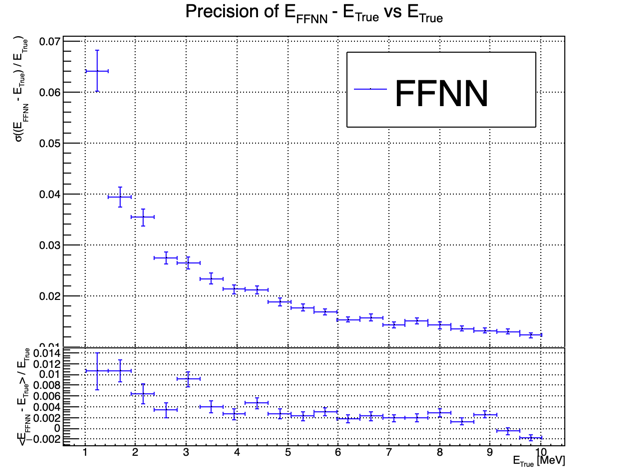
\includegraphics[width=\linewidth]{images/janne/ffnn/ESBE.png}
  \end{subfigure}
  \hfill
  \begin{subfigure}[t]{0.48\linewidth}
    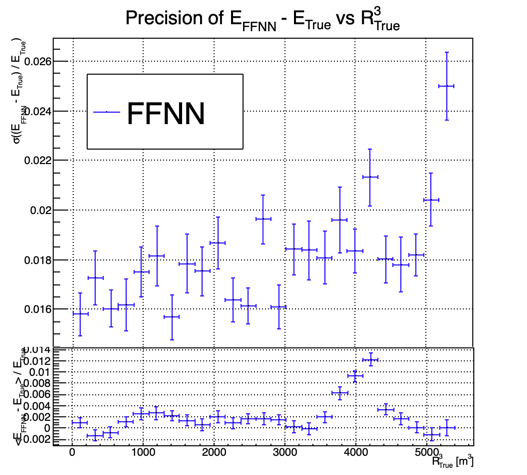
\includegraphics[width=\linewidth]{images/janne/ffnn/ESBR.png}
  \end{subfigure}
  \caption{Energy resolution of the FFNN with respect to the energy (\textbf{On the right}) and the radius (\textbf{On the left})}
  \label{fig:janne:ffnn:ESB}
\end{figure}

\begin{figure}[ht]
  \centering
  \begin{subfigure}[t]{0.48\linewidth}
    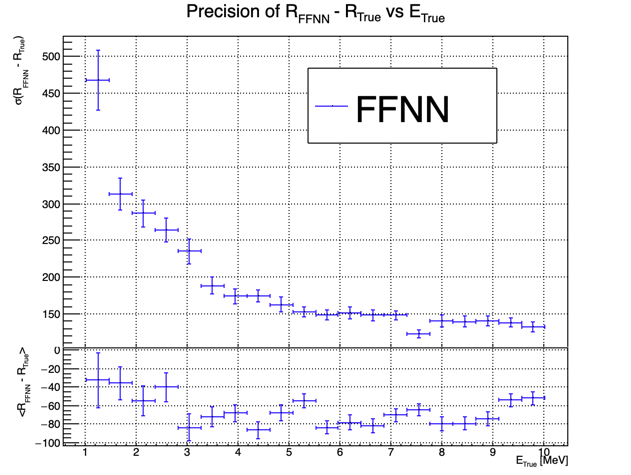
\includegraphics[width=\linewidth]{images/janne/ffnn/SBE.png}
  \end{subfigure}
  \hfill
  \begin{subfigure}[t]{0.48\linewidth}
    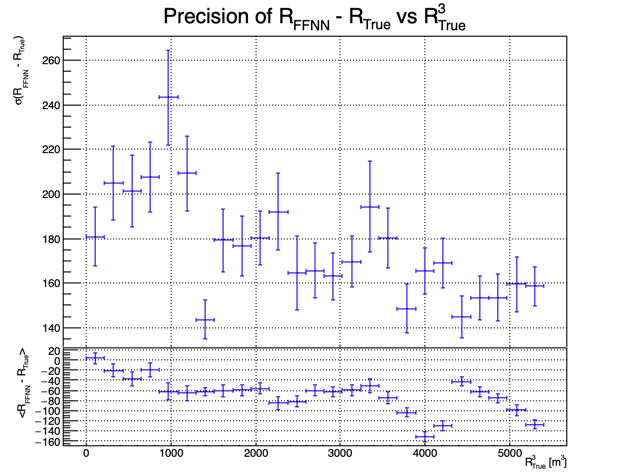
\includegraphics[width=\linewidth]{images/janne/ffnn/SBR.png}
  \end{subfigure}
  \caption{Radial resolution of the FFNN with respect to the energy (\textbf{On the right}) and the radius (\textbf{On the left})}
  \label{fig:janne:ffnn:SB}
\end{figure}

\subsection{Adversarial Neural Network (ANN)}
\label{sec:janne:arch:ann}
%\begin{itemize}
%  \item Decrire l'architecture de l'ANN
%\end{itemize}

The ANN aims to introduce perturbations in the event data in such a way that these perturbations are not detectable in the control dataset while still degrading the energy reconstruction of the IBD dataset. For this purpose, and for the reasons detailed in Section \ref{sec:janne:back_prop}, the ANN operates on the inputs of the reconstruction network presented above, namely the FFNN. During the training, the parameters of the FFNN are \textit{frozen,} meaning they will not be updated during the ANN training. If they were free to be optimized, they would adapt to the perturbations of the ANN, which would go against the objective of this work.

The FFNN takes as input a vector of $5 \times 3072$values, representing the $(x,y,z,Q,t)$ of 3072 Healpix pixels. Those values come from the aggregation of the PMTs belonging to those pixels.

It seems unreasonable that the ANN would modify the pixel positions, as they are derived from a mathematical construction. It could, however, perturb which PMTs are assigned to specific pixels, introducing localization errors, but the position of the PMTs is carefully monitored during JUNO’s construction. Such aggregation errors would likely arise from PMTs located at the edges of the pixels, yet this scenario seems unlikely. Moreover, due to the constraints mentioned in Section \ref{sec:janne:back_prop}, the ANN is required to work with the same format that the FFNN uses as input.


At the start of the project, we attempted to have it operate on both time and charge information simultaneously, but it struggled to converge. After discussions with colleagues in the collaboration, we decided that the ANN would only introduce perturbations in the charge information, as most of the energy information comes from the charge.

Our ANN thus needs to output a 3200-dimensional vector, which represents the updated charges of the detector.

We decided on a Fully Connected Deep NN (DNN) ``bottleneck'' architecture for the ANN, illustrated in Figure \ref{fig:janne:ann_arch}. This architecture places a 4096-neuron-wide layer after the input, followed by smaller layers of sizes 2048, 1024, and 512 neurons, before finally reaching the 256-neuron layer. From this layer, the size increases again to 512, 1024, and finally 2048 neurons before the output layer, which consists of 3072 neurons.


\begin{figure}
  \centering
  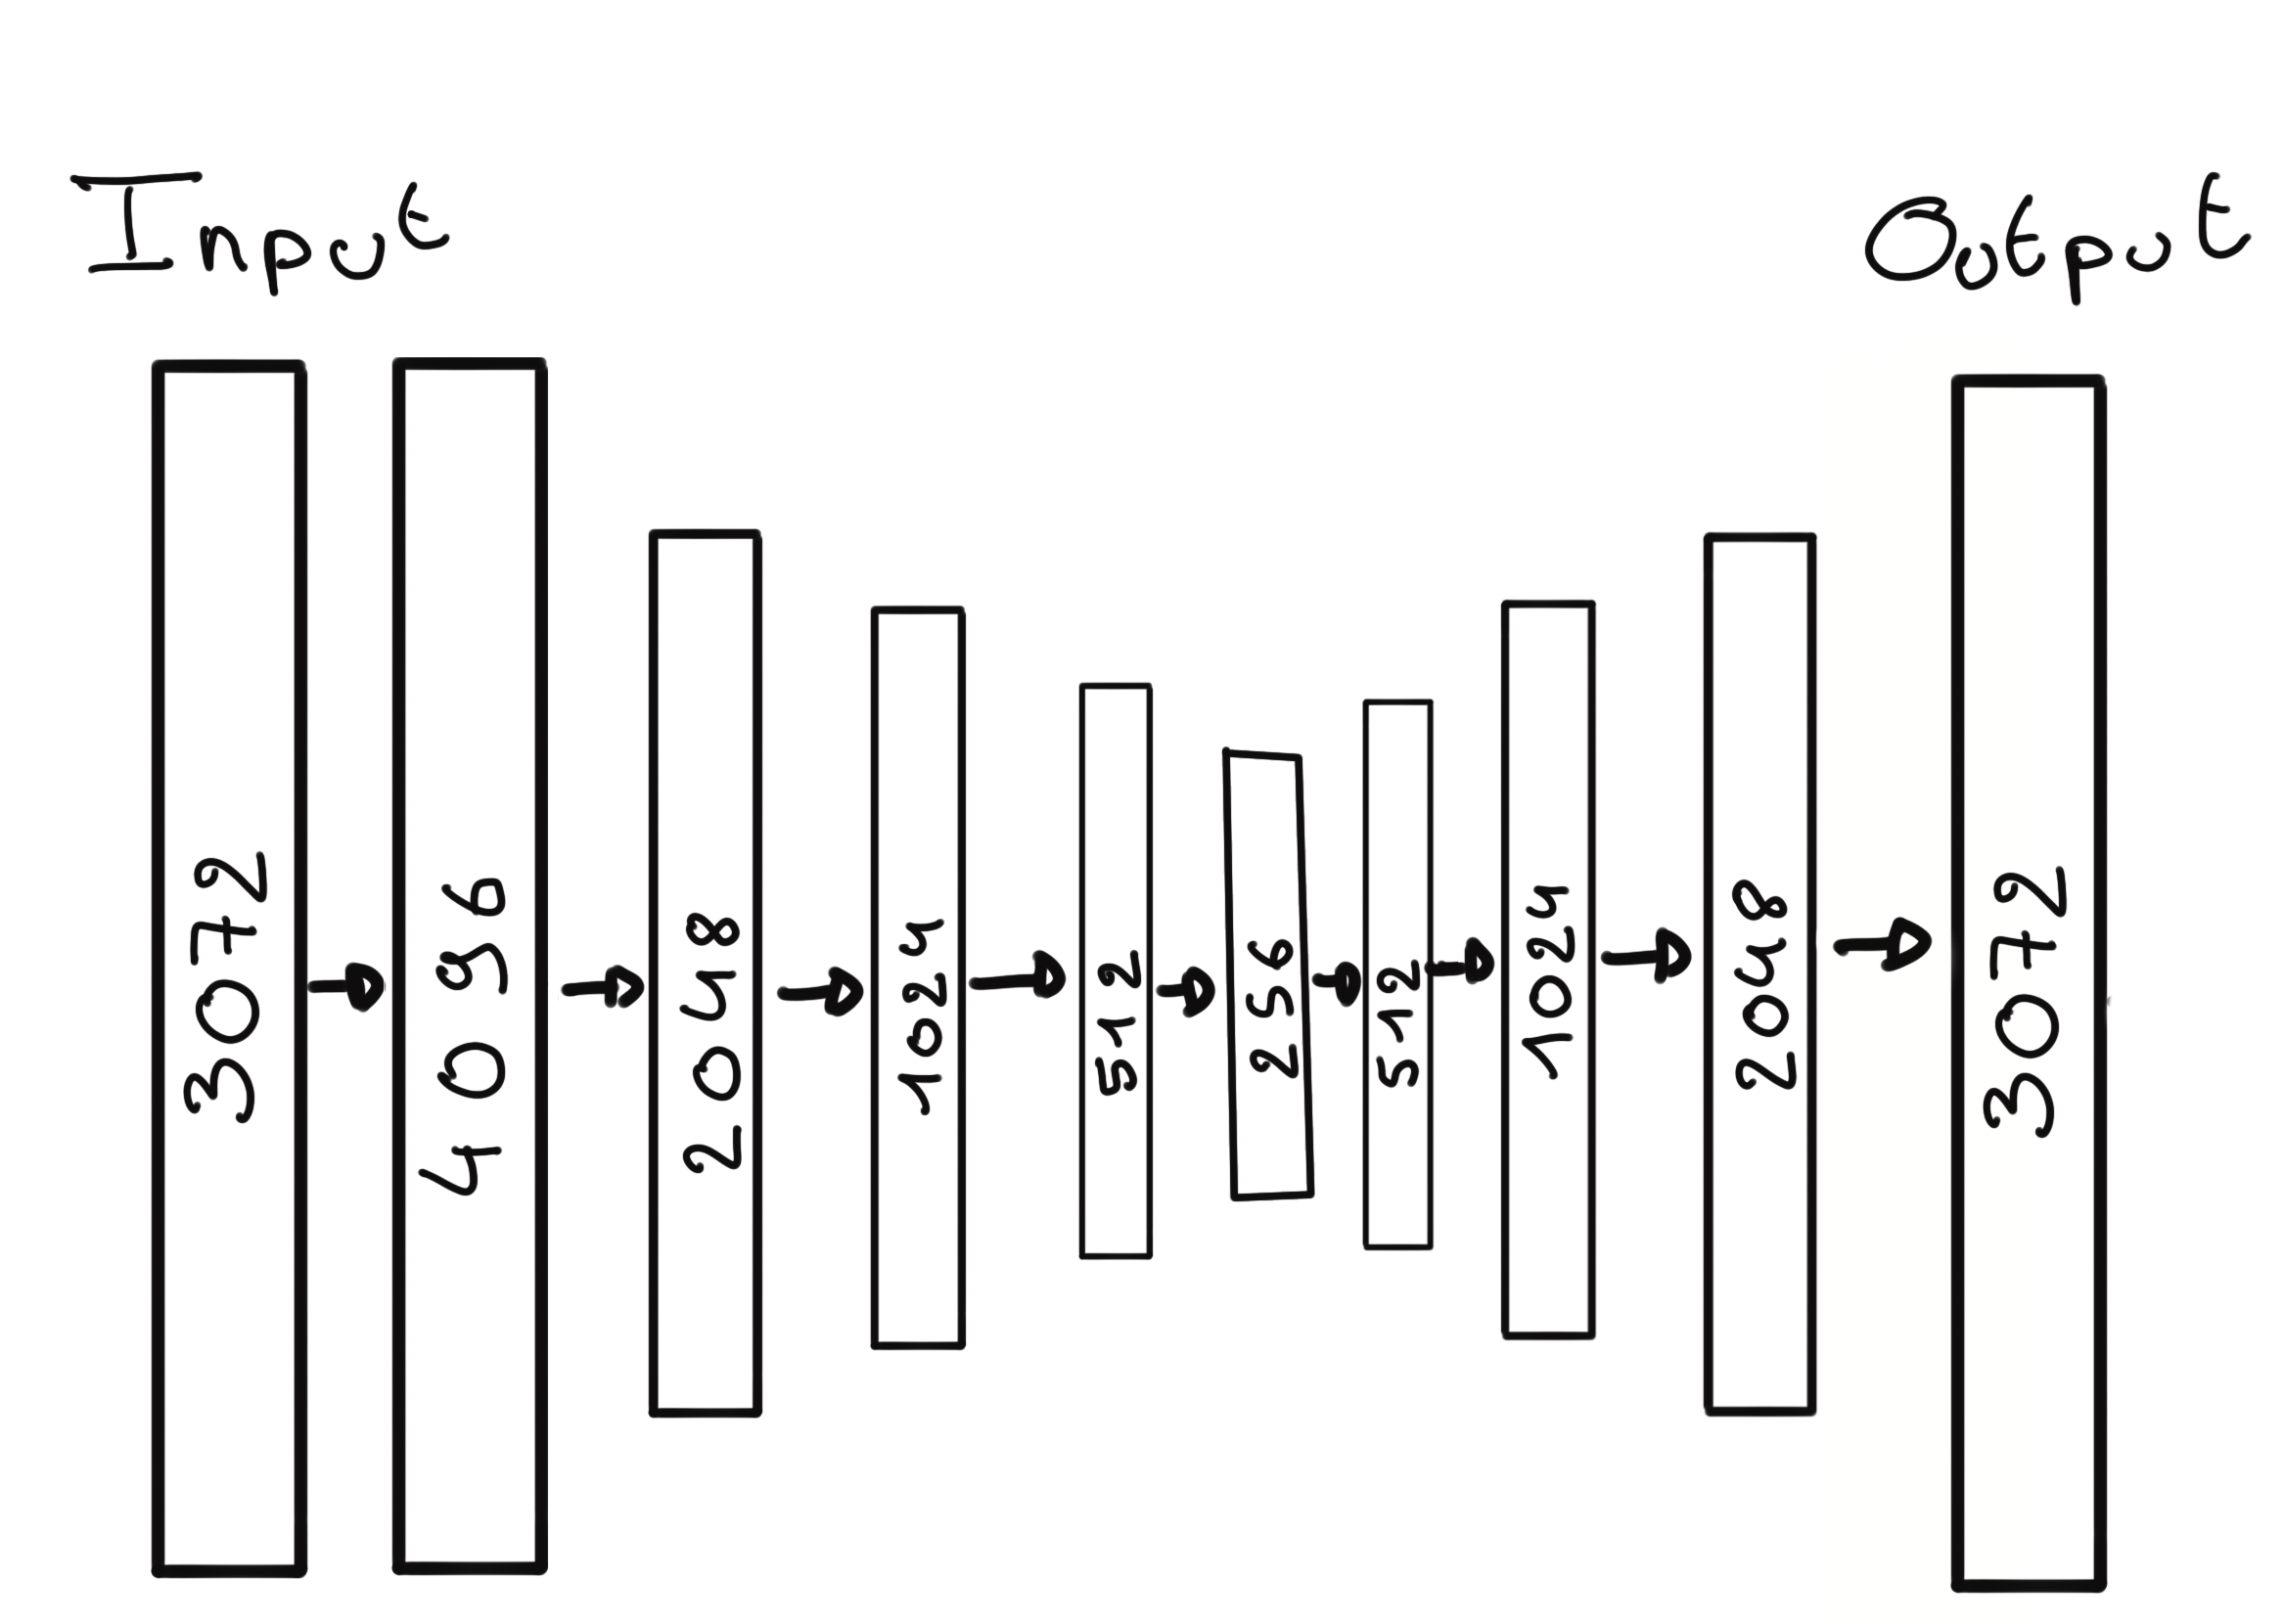
\includegraphics[height=6cm]{images/janne/ANN_illustration.png}
  \caption{Illustration of the ``bottleneck'' architecture of the ANN. Each block represent a fully connected layer with, on the left, the input layer and on the right the output layer. We see a first reduction of the number of neurons per layer, going from 4096 to 256, followed by an augmentation back to 4096 neurons, thus the ``bottleneck''}
  \label{fig:janne:ann_arch}
\end{figure}

The idea behind this architecture is that, by reducing the number of neurons per layer, we force the network to summarize the event in 256 parameters, that it will use to regenerate an event. This architecture has also the advantage of keeping the number of learnable parameters relatively small, as the connection between small layers do not require a lot of parameters.

\subsubsection{ANN loss}

As it was mentioned in the introduction of Section \ref{sec:janne:arch}, the loss of the ANN is composed of two losses, the adversarial loss ${\cal L}_{adv}$ and the regularisation loss ${\cal L}_{reg}$. To those two losses, we adjoin a penalty term that prevent the ANN from producing non-physical events.
\begin{equation*}
  {\cal L} = {\cal L}_{adv} + {\cal L}_{reg} + P
\end{equation*}

The adversarial loss ${\cal L}_{adv}$ is defined as the absolute value correlation between the reconstructed energy and the energy deposit (Eq. \ref{eq:janne:ladv}). The regularisation loss ${\cal L}_{reg}$ is the MSE of the true and reconstructed energy position vector $(x, y, z, E)$ (Eq. \ref{eq:janne:lreg}).

The penalty term is here to prevent the network from generating event that are too far from the initial event. The penalty $P$ is a function that takes the pixelated event $X$, its transformation after the ANN ${\cal G}(X)$ and a constraint $\epsilon$
\begin{equation}
  P(X, {\cal G}(X), \epsilon) = \sum_{i=1}^{3072} \left( ReLU(-{\cal G}(X)_i) + D_i \right)
\end{equation}
with
\begin{equation}
  D_i = \begin{cases}
    \frac{(X_i - {\cal G}(X)_i)^2}{X_i^2}& \text{if } \frac{|X_i - {\cal G}(X)_i|}{X_i} > \epsilon \\
    0& \text{otherwise}
  \end{cases}
\end{equation}
where $i$ index the Healpix pixels. The term $ReLU(-{\cal G}(X)_i$ is minimal, equal 0, when the charge after perturbation is positive. This term prevent the ANN from producing negative charge, feat impossible for the PMTs.

The second term $D_i$ is equal to 0 when the relative charge between the original and perturbed pixel is less than $\epsilon$. Otherwise, it is the square of this relative charge difference. This term penalize the ANN from producing charges too different from the original event.
\hfill

When dealing with multiple losses like this, it is important keep then of the same order of magnitude, as we do not want one term to absorb the other.

The loss ${\cal L}_{adv}$ range from 0 to 1 while ${\cal L}_{reg}$ is 0 when the vertex is perfectly reconstructed by it can theoretically go up to infinity. In practice we expect it to take value of the order of magnitude coherent with the reconstruction performances. In fact, if it would take higher value, it would mean that the reconstruction would reconstruct the event far away from the true vertex in comparison to the expected performance. This kind of issue would be immediately be detected, even with simplistic reconstructions such as the charge barycenter, which goes against the goal of producing subtle fluctuation.

We evaluate ${\cal L}_{reg}$ with $(x, y, z)$ in meter and $E$ in MeV. If the event is reconstructed with a precision of 15 cm and an energy resolution of 3\% at 1 MeV, taking the reconstruction performance of the best reconstruction algorithm OMILREC (see Sections \ref{sec:juno:reco} and \ref{sec:jgnn:results}), ${\cal L}_{reg} \approx 0.3^2 + 0.03^2 = 0.0909$. We see about an order of magnitude between ${\cal L}_{adv}$ and ${\cal L}_{reg}$. To compensate for it we weight ${\cal L}_{reg}$
\begin{equation}
  {\cal L} = {\cal L}_{adv} + 60\cdot{\cal L}_{reg} + P(\epsilon)
\end{equation}

The amplitude of $P$ and the value of $\epsilon$ will be further discussed in Section \ref{sec:janne:arch:training}.

\subsubsection{Hyperparameter optimization}
%\label{sec:janne:arch:hyper}
%\begin{itemize}
%  \item Pour les meme raison que l'ANN:
%    \begin{itemize}
%      \item Phase exploratoire, architecture tres changeante, random search n'est pas viable
%      \item Architecture consomme beaucoup, besoin d'entrainer sur l'A100
%      \item Possiblement que de l'optimization permetterais de faire passer sur V100, mais developement techniques necessaires.
%    \end{itemize}
%\end{itemize}

All the ANN hyperparameters presented above have been optimized through the numerous iteration the architecture went through. The training is computationally expensive as we need to host both networks on the GPU card, reaching quickly the memory limit of the GPU. The training of the ANN can takes up to 90h. The requirement of having a powerful GPU can be met locally, as Subatech possess an available A100 \cite{noauthor_nvidia_nodate-1} card with 40GB of memory. We could not port over computing center as they only possess V100 \cite{noauthor_nvidia_nodate-2} GPU with 20GB of memory.

Those constraint made a random search optimization impossible. It is maybe possible, through optimisation, to reduce the memory requirements to reach the threshold to run on V100 but the challenge was deemed not worth it for an exploratory work.

\section{Training of the ANN}
\label{sec:janne:arch:training}
%\begin{itemize}
%  \item Presentation du dataset
%  \item 2 etapes d'entrainement
%  \item Retour à l'identitié -> que l'ANN ne fasse pas n'importe quoi
%  \item Cassage de la reconstruction
%\end{itemize}

The training of the ANN goes through two phases. The first one consist on reproducing physical events, the second one into searching for physically sound perturbations. For both phases, we use the both of the datasets presented in section \ref{sec:janne:method}. We use a batch size of 64 for both datasets meaning that, for each steps, the network see 128 events.

Each epochs goes through the entirety of the training dataset.

\subsection{First training phase: back to physics}
\label{sec:janne:results:identity}

When the ANN is initialized, before any training has been done, its parameters are initialized with random values. Multiple initialization methods exist. In this work, we use a common He initialization \cite{he_delving_2015}, which is the default initialization in the PyTorch \cite{ansel_pytorch_2024} library. If we were to ask for an event from the ANN without training first, the results would be random noise. We thus first have the ANN learn to reproduce physical events.

For this, we conduct a training of 200 epochs where the loss consists only of the penalty term. For scaling purposes, the penalty $P$ is scaled by 0.25.
\begin{equation}
  {\cal L}_1 = 0.25 \cdot P(\epsilon = 0.01)
\end{equation}
During this phase, the only objective of the network is to yield events that are the same as the original events.


The evolution of this loss ${\cal L}_1$ during the training for the training dataset and the validation dataset is presented in Figure \ref{fig:jann:train:phase_1}.
\begin{figure}[ht]
  \centering
  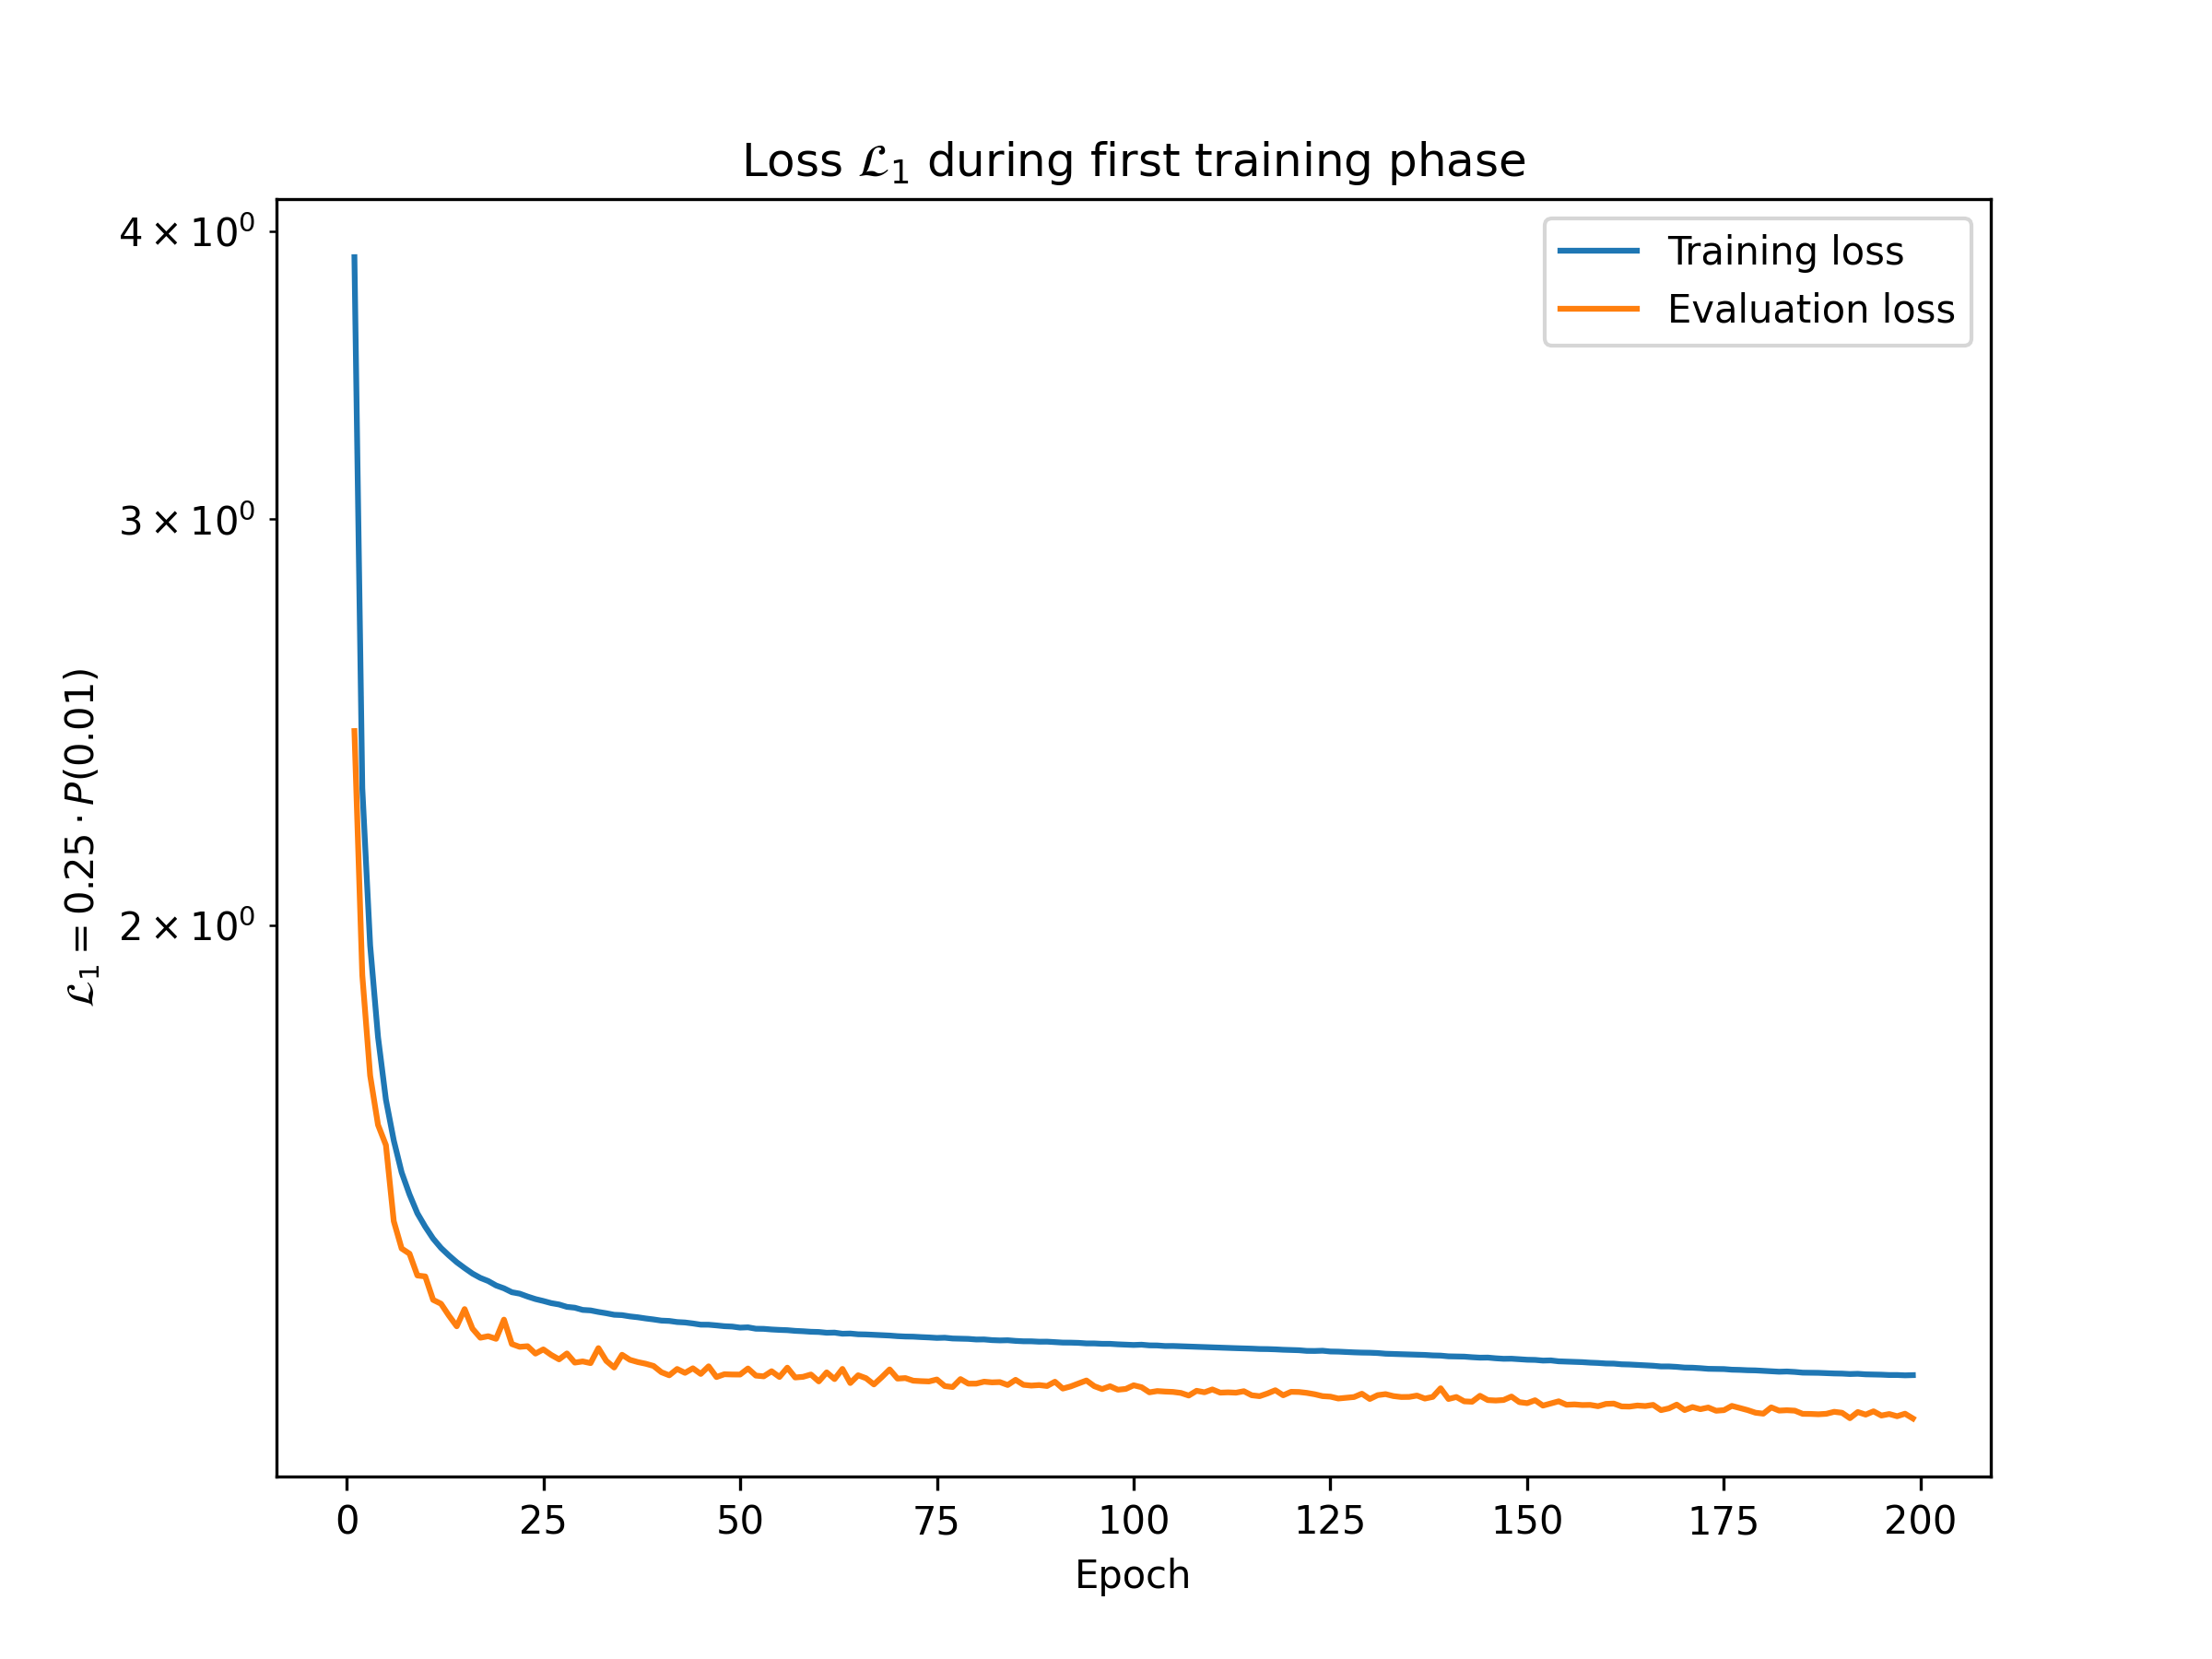
\includegraphics[height=6cm]{images/janne/training/phase_1_penal.png}
  \caption{Evolution of the loss ${\cal L}_1 = 0.25 \cdot P(0.01)$ during the first phase of the training}
  \label{fig:jann:train:phase_1}
\end{figure}
We see that the ANN converges to some stability in the loss.

The time and charge channels of two events, after this training phase, are presented in Figures \ref{fig:janne:hr_he_200} and \ref{fig:janne:lr_le_200}. We remind that the ANN only act on the charge channel of the event.
\begin{figure}[ht]
  \centering
  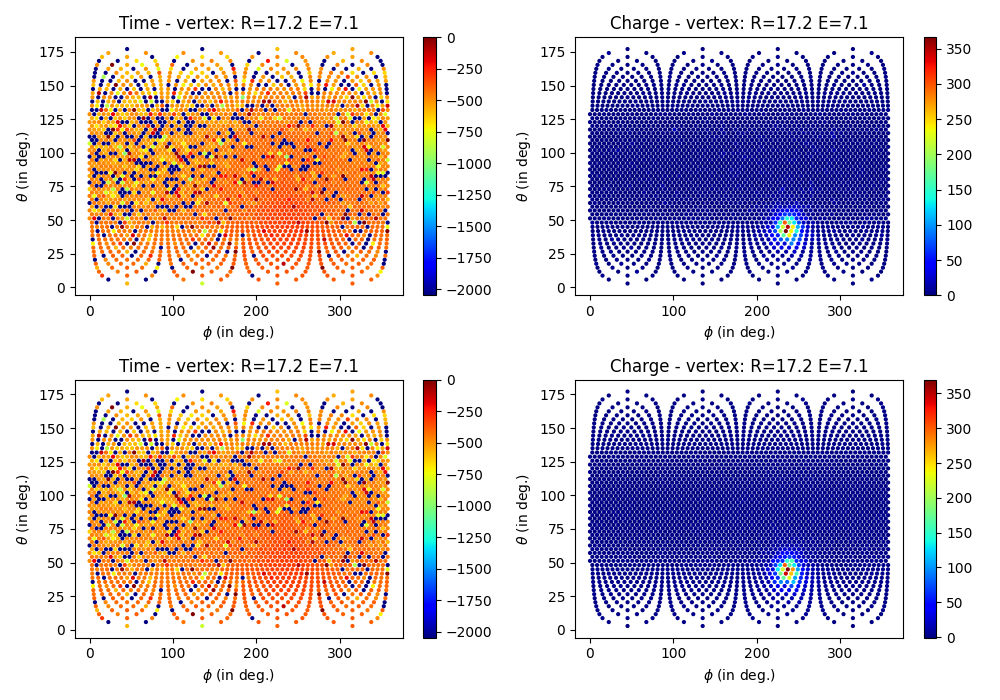
\includegraphics[height=7cm]{images/janne/events/hr_he_200.png}
  \caption{Time channel (on the left) and charge channel (on the right) of a \textbf{radial, high energy event} ($R$ = 17.2 m, $E_{dep}$ = 7.1 MeV), \textbf{Top:} before the ANN perturbation, \textbf{Bottom:} after the ANN perturbation. The ANN have been trained for 200 epochs, just after Phase 1. Time channel in ns and charge channel in $N_{pe}$.}
  \label{fig:janne:hr_he_200}
\end{figure}

\begin{figure}[ht]
  \centering
  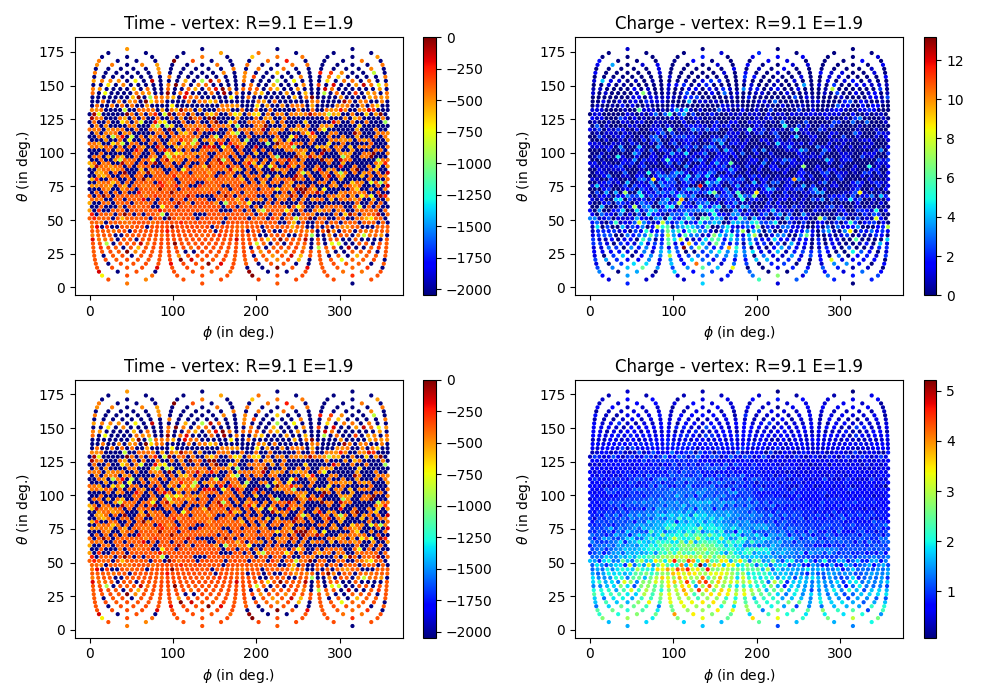
\includegraphics[height=7cm]{images/janne/events/lr_le_200.png}
  \caption{Time channel (on the left) and charge channel (on the right) of a \textbf{central, low energy event} ($R$ = 9.1 m, $E_{dep}$ = 1.9 MeV), \textbf{Top:} before the ANN perturbation, \textbf{Bottom:} after the ANN perturbation. The ANN have been trained for 200 epochs, just after Phase 1. Time channel in ns and charge channel in $N_{pe}$.}
  \label{fig:janne:lr_le_200}
\end{figure}

We observe that for a localized event, Figure \ref{fig:janne:hr_he_200}, the ANN correctly reproduces the event, while for a more diffuse event, Figure \ref{fig:janne:lr_le_200}, it produces a more uniform charge distribution. By looking at the color scale in Figure \ref{fig:janne:lr_le_200}, we observe that the ANN does not reproduce singular high numbers of $N_{pe}$. The highest pixel in the original was 12 $N_{pe}$, whereas after the ANN, the highest pixel is 5 $N_{pe}$. Furthermore, whereas in the original event the charge repartition, while diffuse, was still concentrated in specific pixels, the ANN spreads the charges in all the pixels.

In the next figures, we discuss the reconstruction of the FFNN (${\cal F}$) with and without the presence of the ANN $({\cal G})$ at the end of this Phase 1. The reconstruction by the FFNN of an event perturbed by the ANN is denoted $({\cal F} \circ {\cal G})$. We differentiate the reconstruction between the two datasets, presented in Section \ref{sec:janne:method}: the physics dataset, designated as IBD, and the control dataset, designated $^{12}B$.

In Figure \ref{fig:janne:f_circ_over_f_200}, we show the ratio between the reconstructed energy distribution before and after the application of the ANN. For the $^{12}$B dataset, the ratio is close to one except in the bin $E_{rec} > 9.5$ MeV, where we see an excess of events after the ANN. For the IBD dataset, the ratio is close to 1 over the energy range.

\begin{figure}[ht]
  \centering
  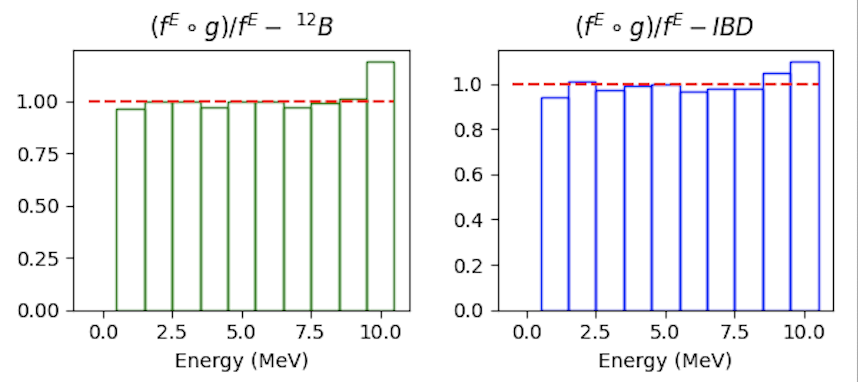
\includegraphics[height=4cm]{images/janne/f_circ_over_f_200.png}
  \caption{Ratio of the reconstructed energy spectra between $({\cal F} \circ {\cal G})$ and ${\cal F}$ at then end of Phase 1 of the training. \textbf{On the left :} For the $^{12}$B dataset. \textbf{On the right :} For the IBD dataset}
  \label{fig:janne:f_circ_over_f_200}
\end{figure}

In Figure \ref{fig:janne:rec_err_200}, we present the distribution of the relative reconstruction errors $(E_{rec}, E_{dep})/E_{dep})$ with (light histogram) and without (dark histogram) the ANN. We see that without the ANN, the distribution was centered on 0, whereas with it, we observe a small positive bias. In the second row of the histogram, the ratio between the light and dark histograms, we see confirmation of the previous observation, with a deficit of events for $-0.05 < (E_{rec}, E_{dep})/E_{dep}) < 0.02$ and an excess of events for $(E_{rec}, E_{dep})/E_{dep}) > 0.02$. This shift to higher energy explains the excess of events seen in the highest energy bins in Fig. \ref{fig:janne:f_circ_over_f_200}.

The behavior between the $^{12}$B dataset (green histogram) and the IBD dataset (blue histogram) is similar.
\begin{figure}[ht]
  \centering
  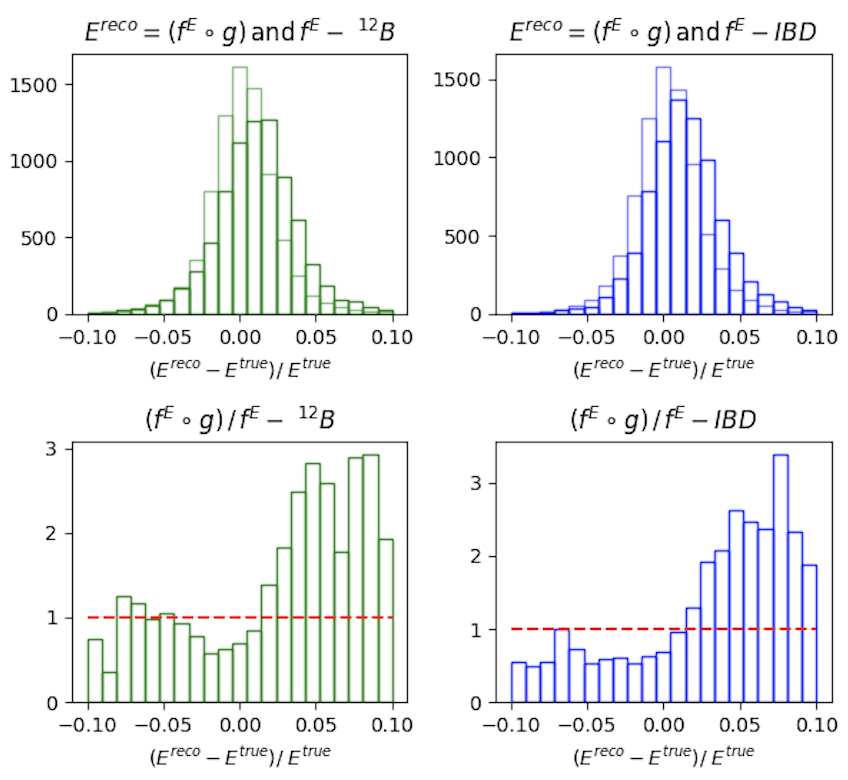
\includegraphics[height=8cm]{images/janne/rec_err_200.png}
  \caption{\textbf{On the top :} Distribution of the relative energy reconstruction error between ${\cal F}$ (light histogram) and $({\cal F} \circ {\cal G})$ (dark histogram) at then end of Phase 1 of the training. \textbf{On the bottom :} Ratio between the light and dark histogram of the top figure.}
  \label{fig:janne:rec_err_200}
\end{figure}


\subsection{Second training phase: Breaking of the reconstruction}
\label{sec:janne:results:break}

Once the ANN is able to reproduce physical events, we change the loss so that it starts to search for potential perturbations.
For this we introduce the term ${\cal L}_{adv}$ and ${\cal L}_{red}$ producing a second loss ${\cal L}_2$.
Adding those terms will significantly change the loss.
The previous minima in the parameter phase space the ANN found minimizing ${\cal L}_1$ will not be the minima ${\cal L}_2$. To prevent a gradient explosion, we introduce a growing factor $\lambda$ in front of the term ${\cal L}_{adv}$ and ${\cal L}_{red}$. This factor starts at $\lambda  = 0.01$ at epoch 201 and grows $\lambda_{i+1} = \lambda_{i} + 0.01$ where $i$ indexes the epoch. It caps at $\lambda_{max} = 1$ at epoch 300 after which it stops growing.

Also to ease the task of the ANN, we relax the constraint in the penalty term $P$ from $P(0.01)$ to $P(0.15)$.

The expression of the phase 2 loss ${\cal L}_2$ becomes:
\begin{equation}
  \label{eq:janne:phase_2:loss}
  {\cal L}_2 = \lambda \left( {\cal L}_{adv} + 60 \cdot {\cal L}_{reg} \right) + 0.25 \cdot P(0.15)
\end{equation}


This second phase of the training last for 200 more epochs, up to epoch 400.

The profiles of ${\cal L}_2$, ${\cal L}_{adv}$, $60 \cdot {\cal L}_{reg}$ and $0.25 \cdot P(0.15)$ during this second phase of the training are presented in Figures \ref{fig:janne:phase_2_1} and \ref{fig:janne:phase_2_2}. The profile of the loss ${\cal L}$ over entirety of the training is presented in figure \ref{fig:janne:phase_all}.

\begin{figure}
  \centering
  \begin{subfigure}[t]{0.48\linewidth}
    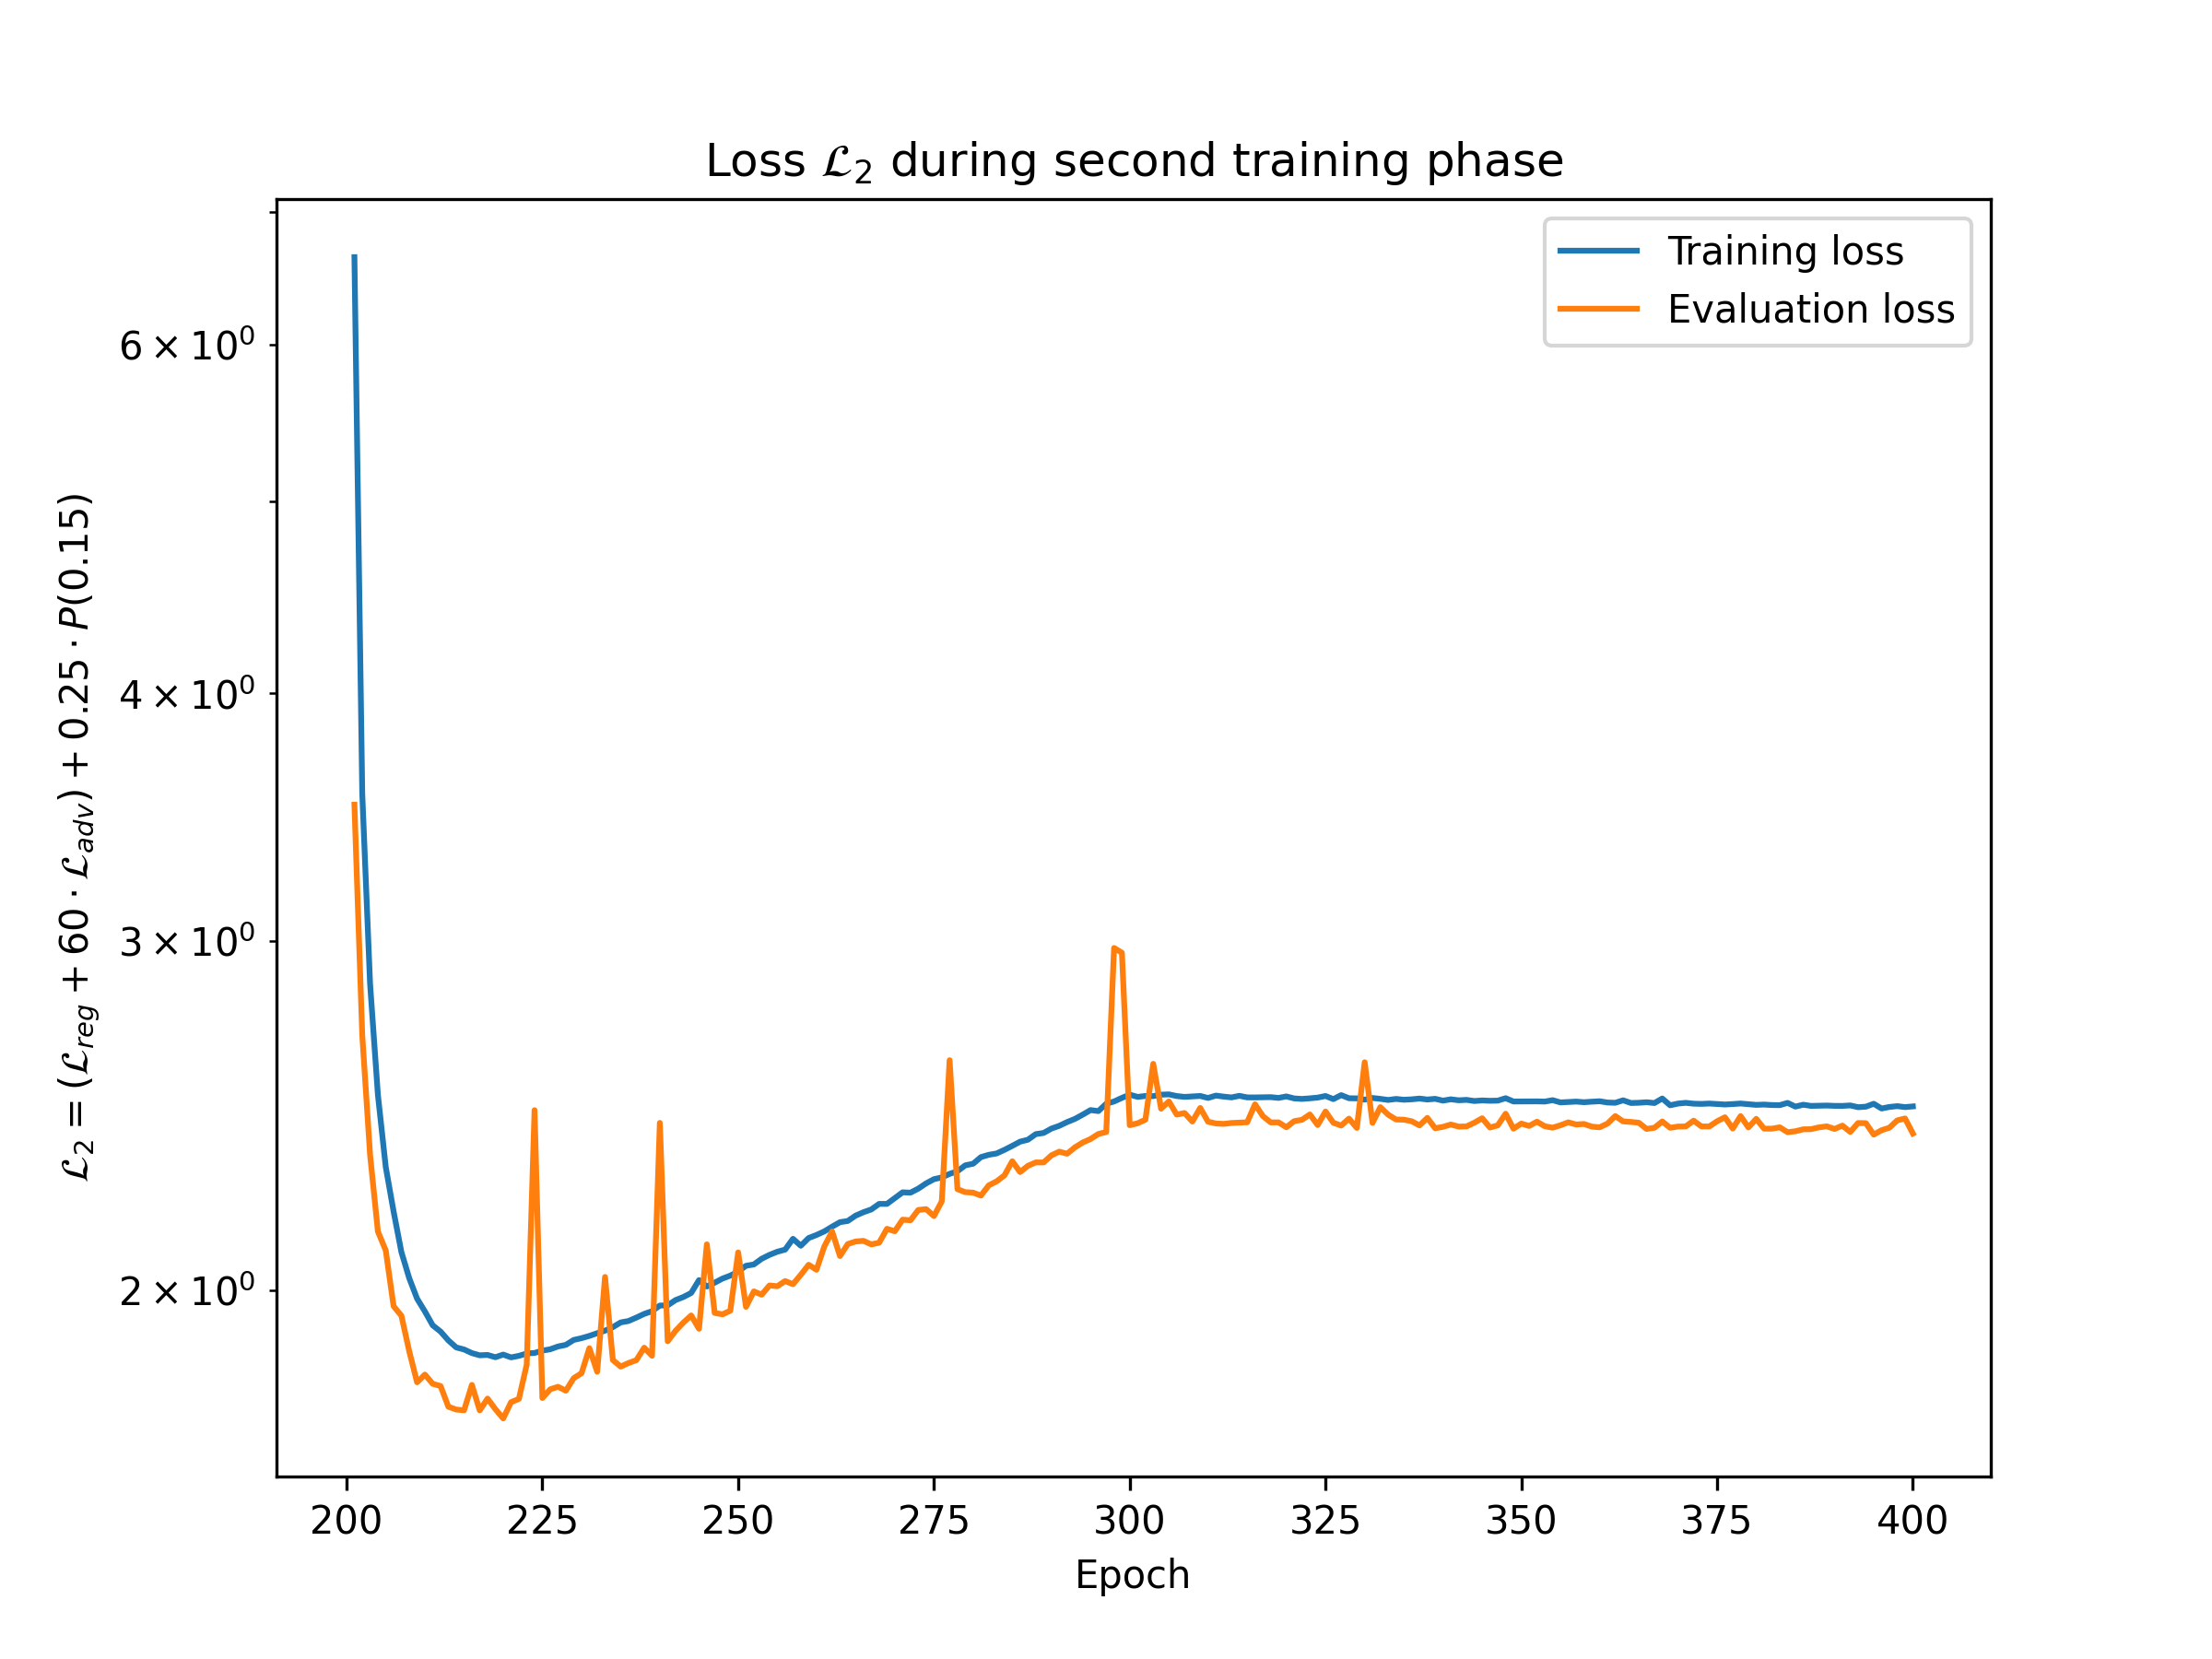
\includegraphics[width=\linewidth]{images/janne/training/phase_2_loss.png}
  \end{subfigure}
  \hfill
  \begin{subfigure}[t]{0.48\linewidth}
    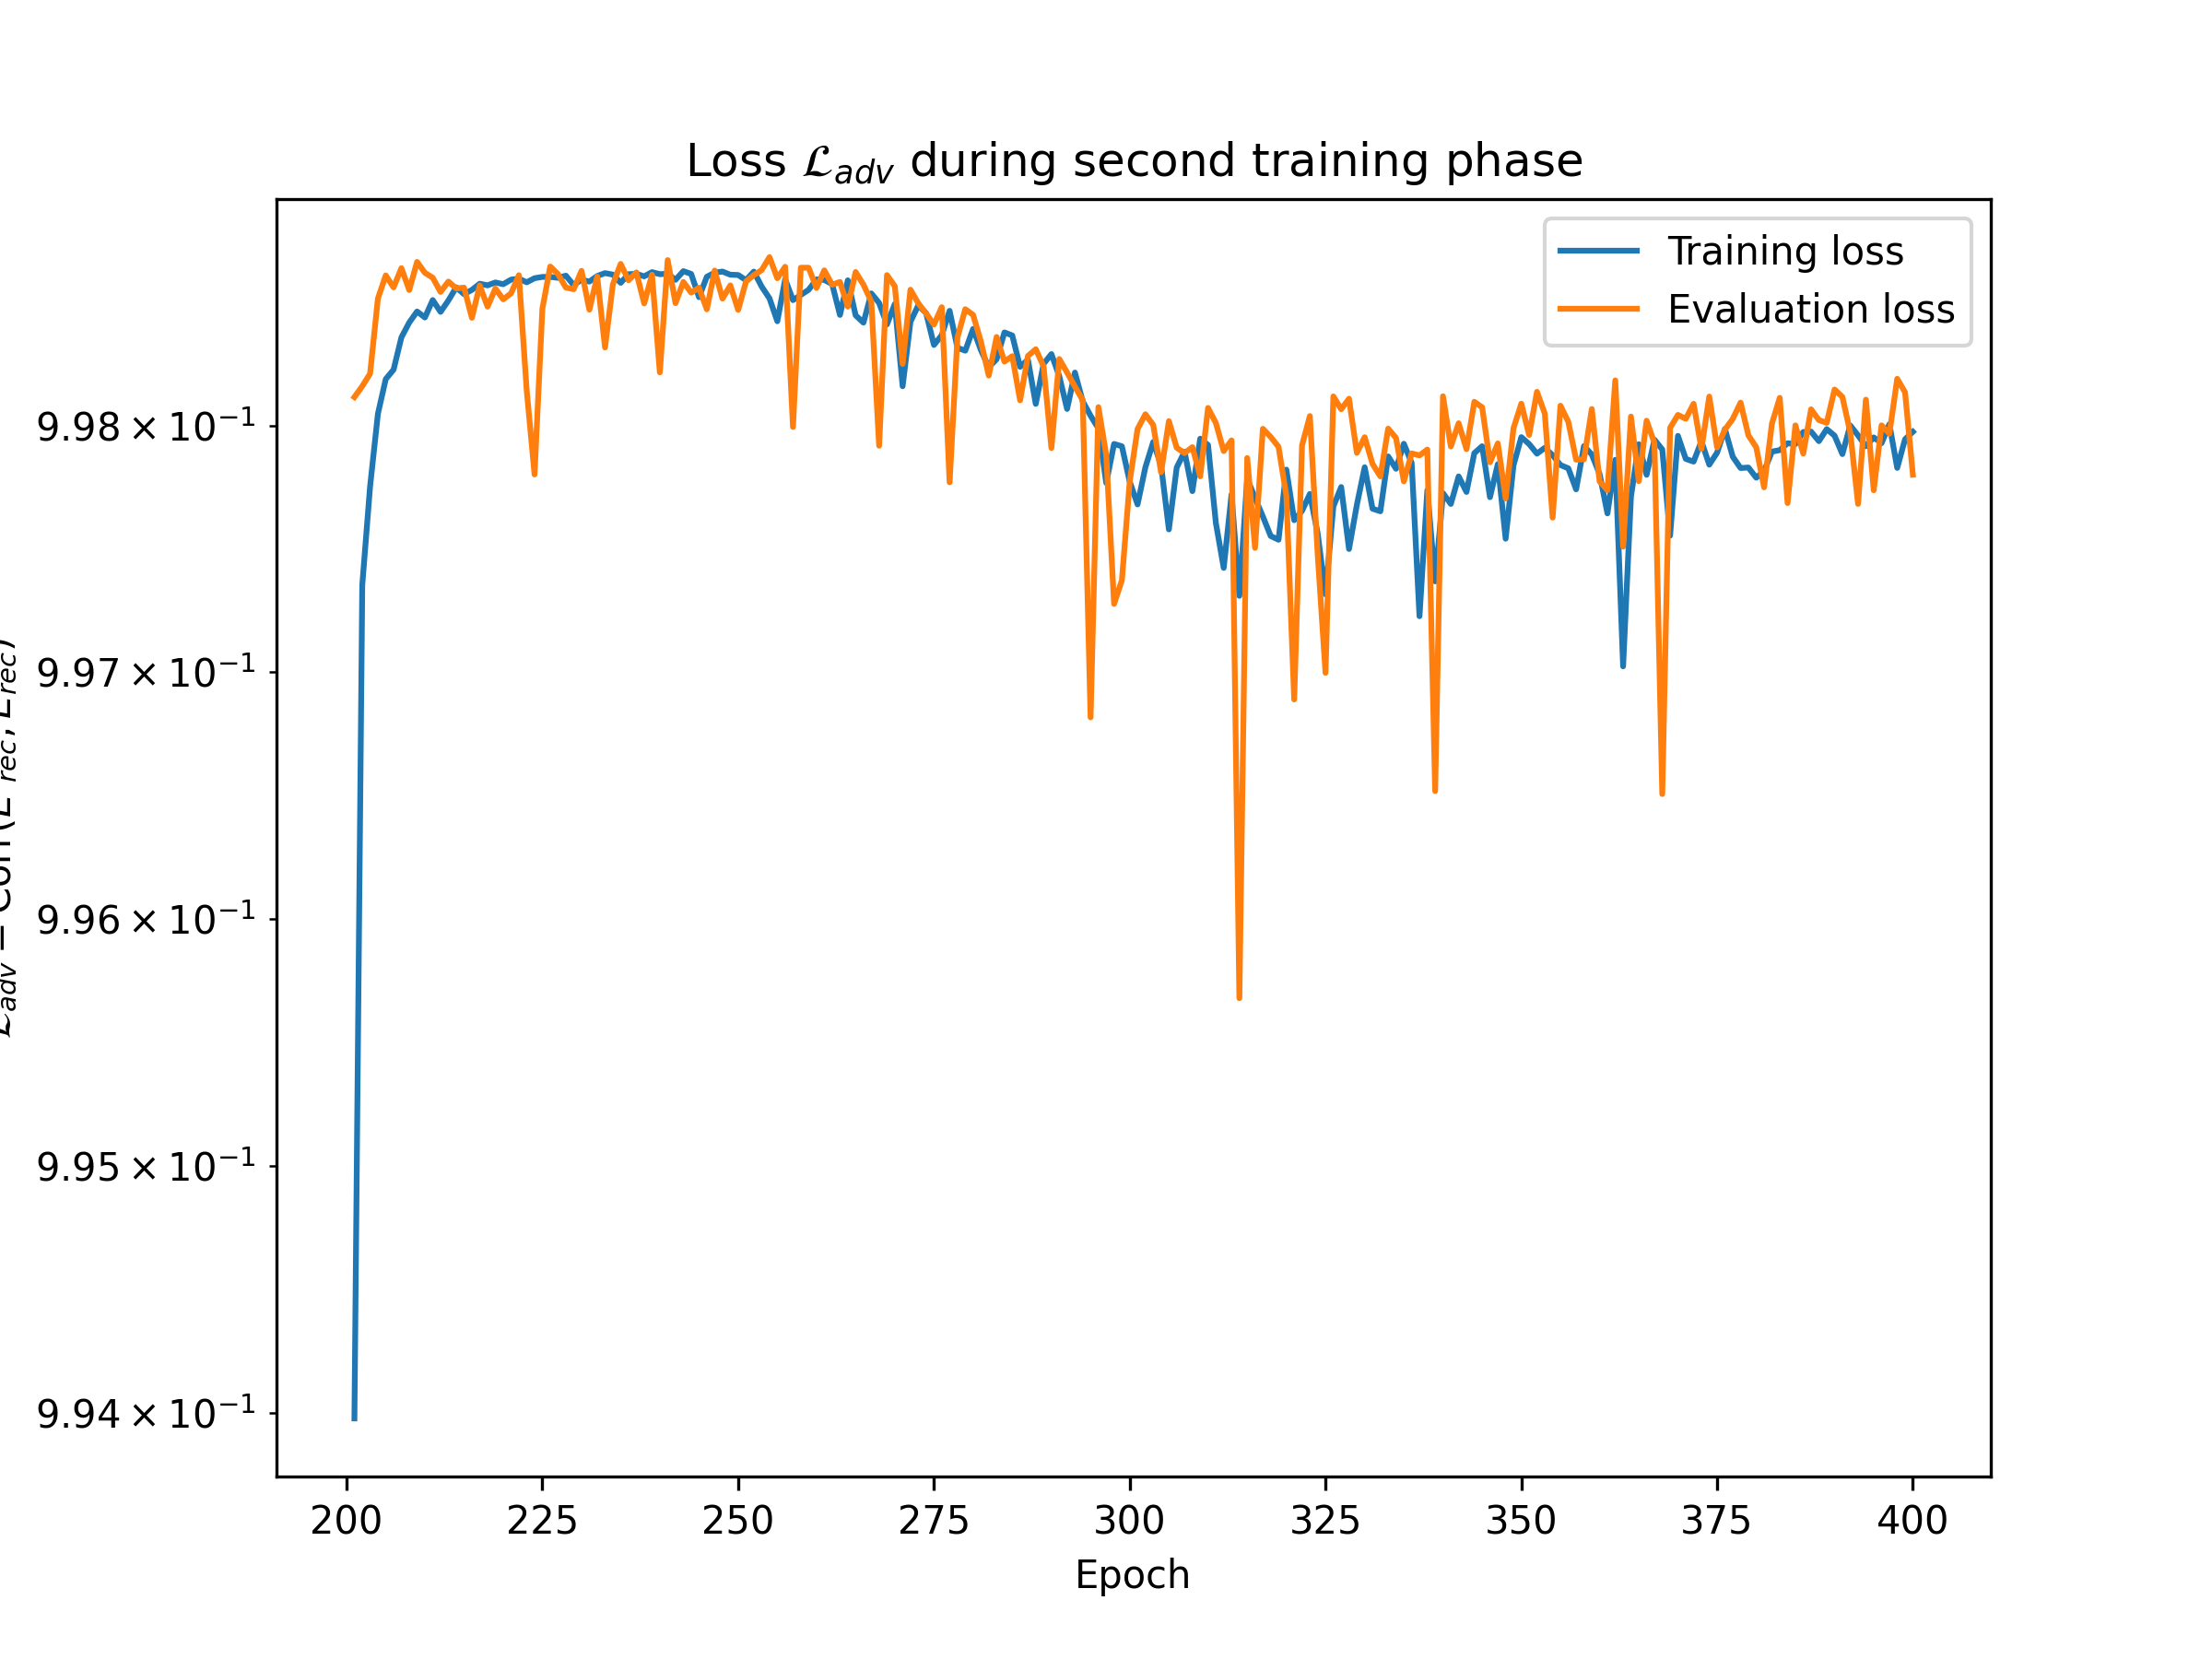
\includegraphics[width=\linewidth]{images/janne/training/phase_2_loss_adv.png}
  \end{subfigure}
  \caption{Profile of the loss ${\cal L}_2$ and ${\cal L}_{adv}$ during the second phase of training. The linear increase of ${\cal L}_2$ is due to the growing factor $\lambda$ in Eq. \ref{eq:janne:phase_2:loss}.}
  \label{fig:janne:phase_2_1}
\end{figure}

\begin{figure}
  \centering
  \begin{subfigure}[t]{0.48\linewidth}
    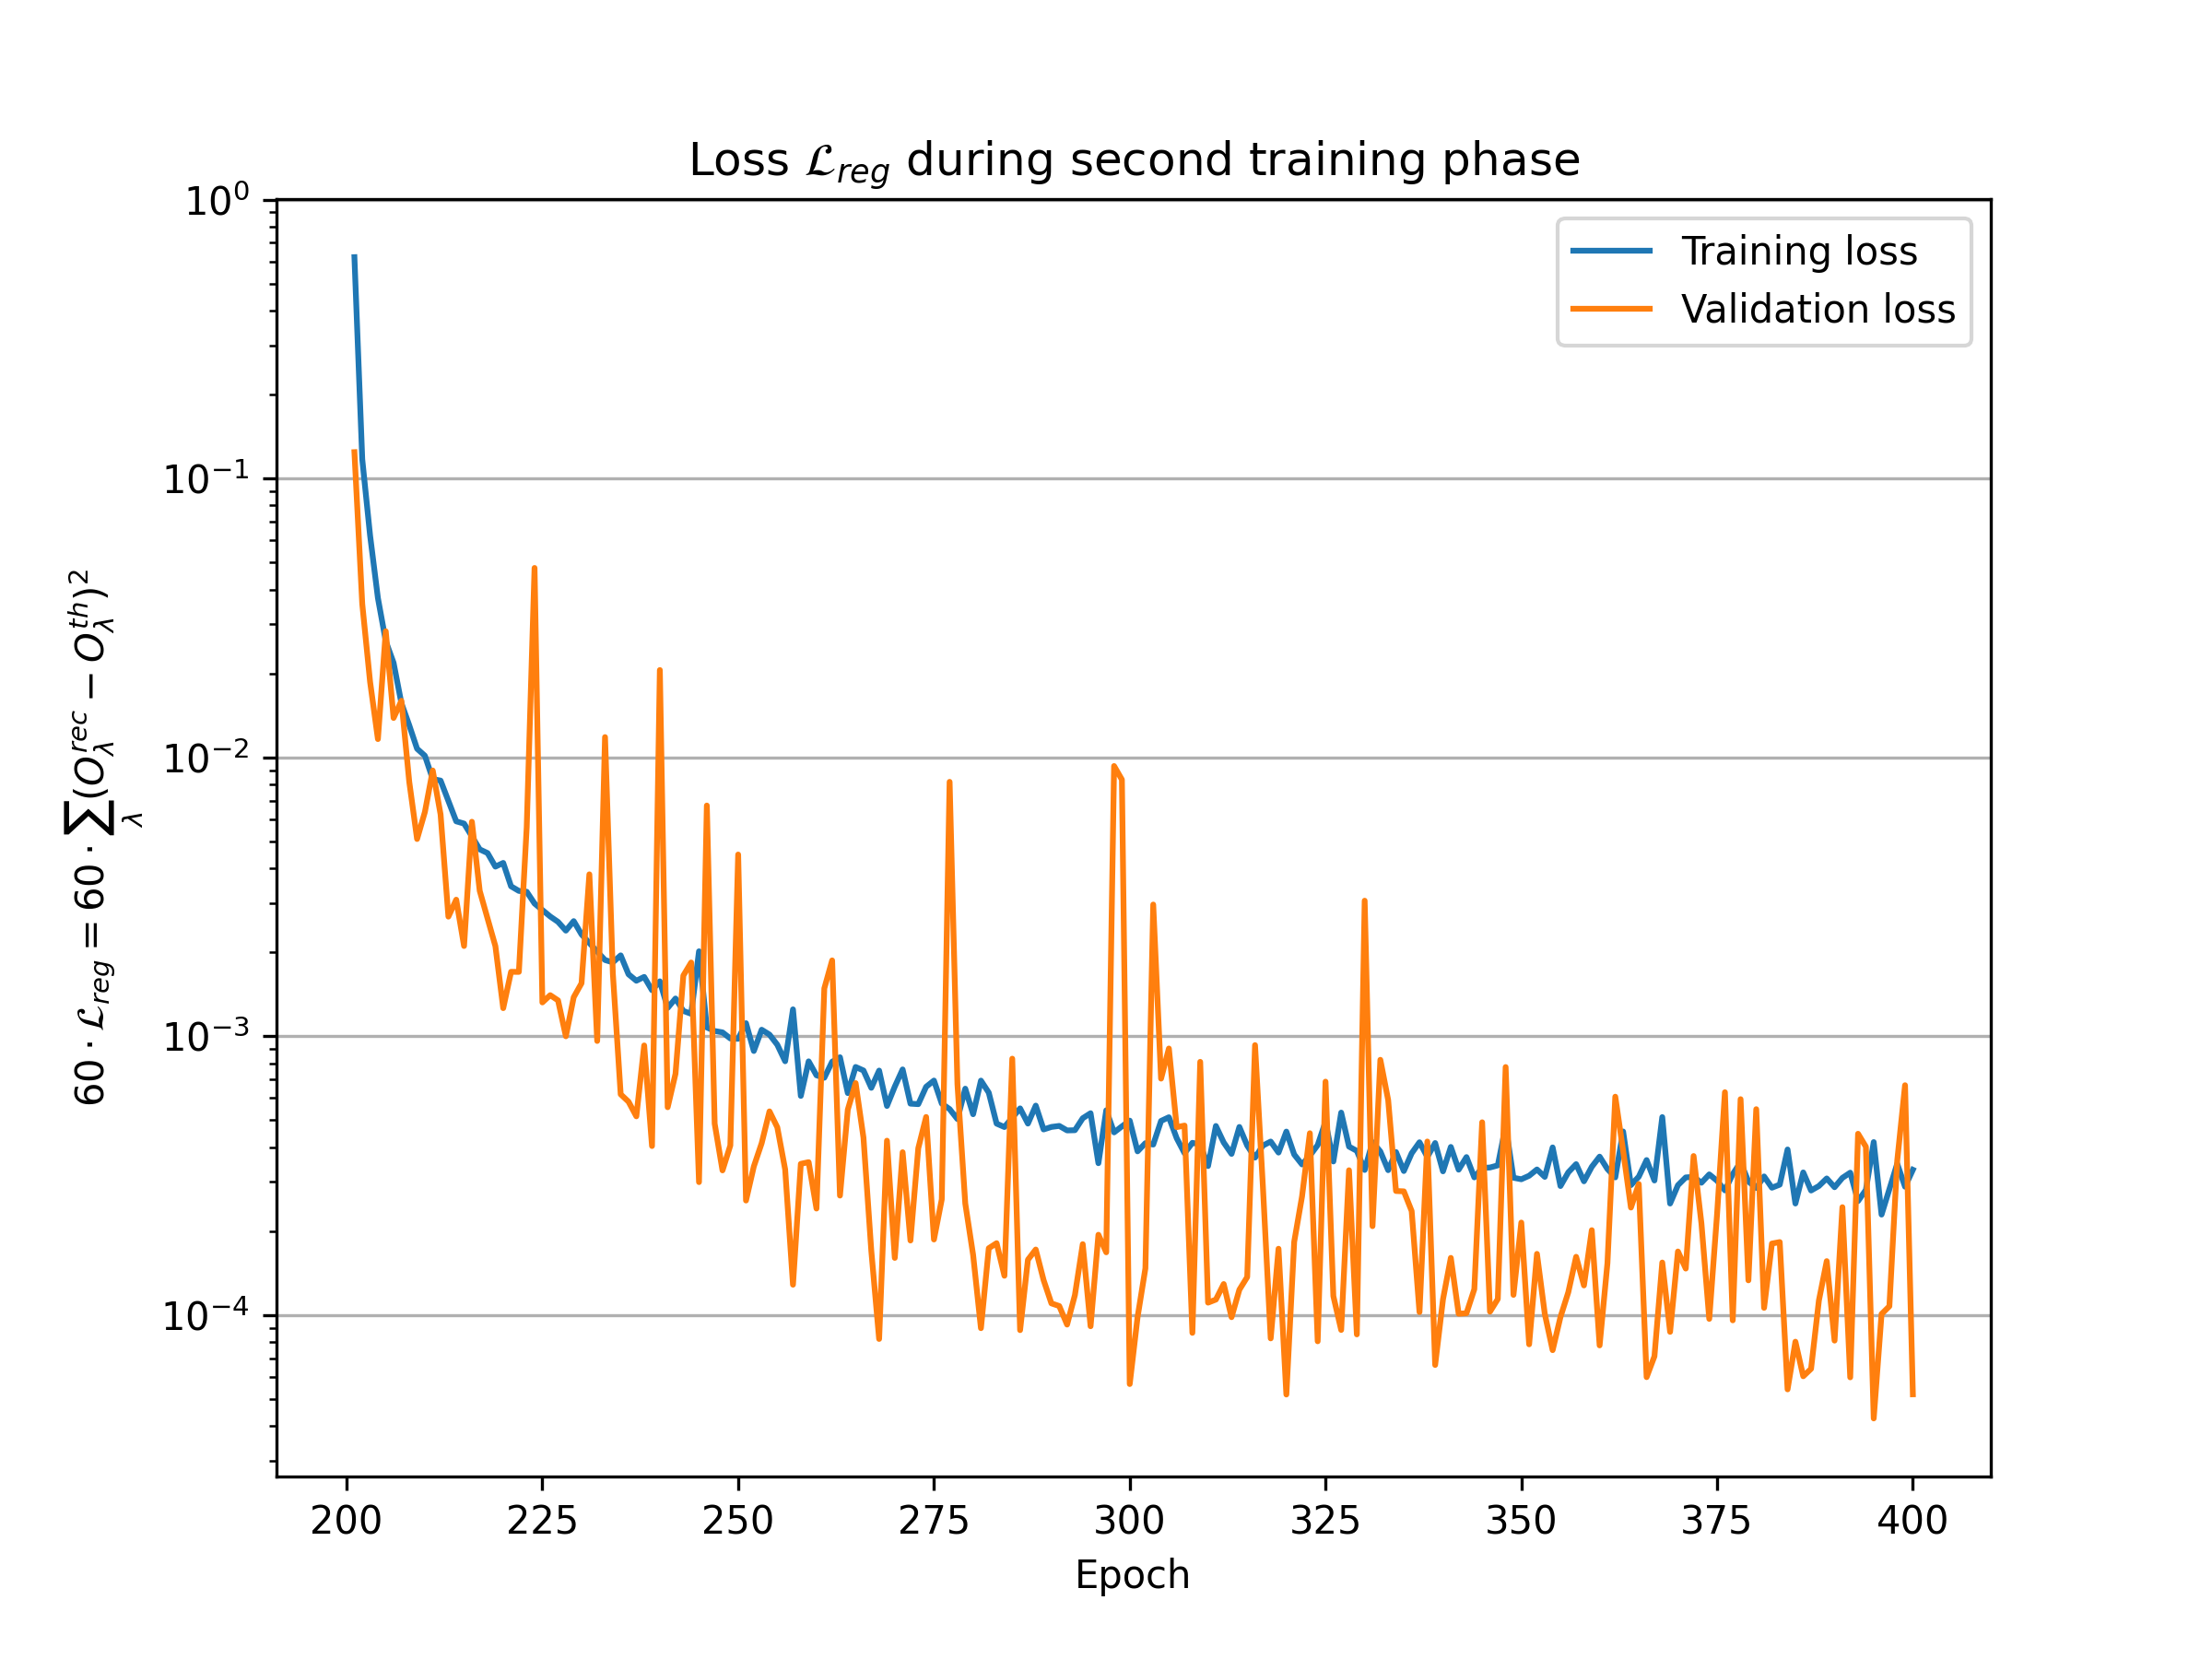
\includegraphics[width=\linewidth]{images/janne/training/phase_2_loss_reg.png}
  \end{subfigure}
  \hfill
  \begin{subfigure}[t]{0.48\linewidth}
    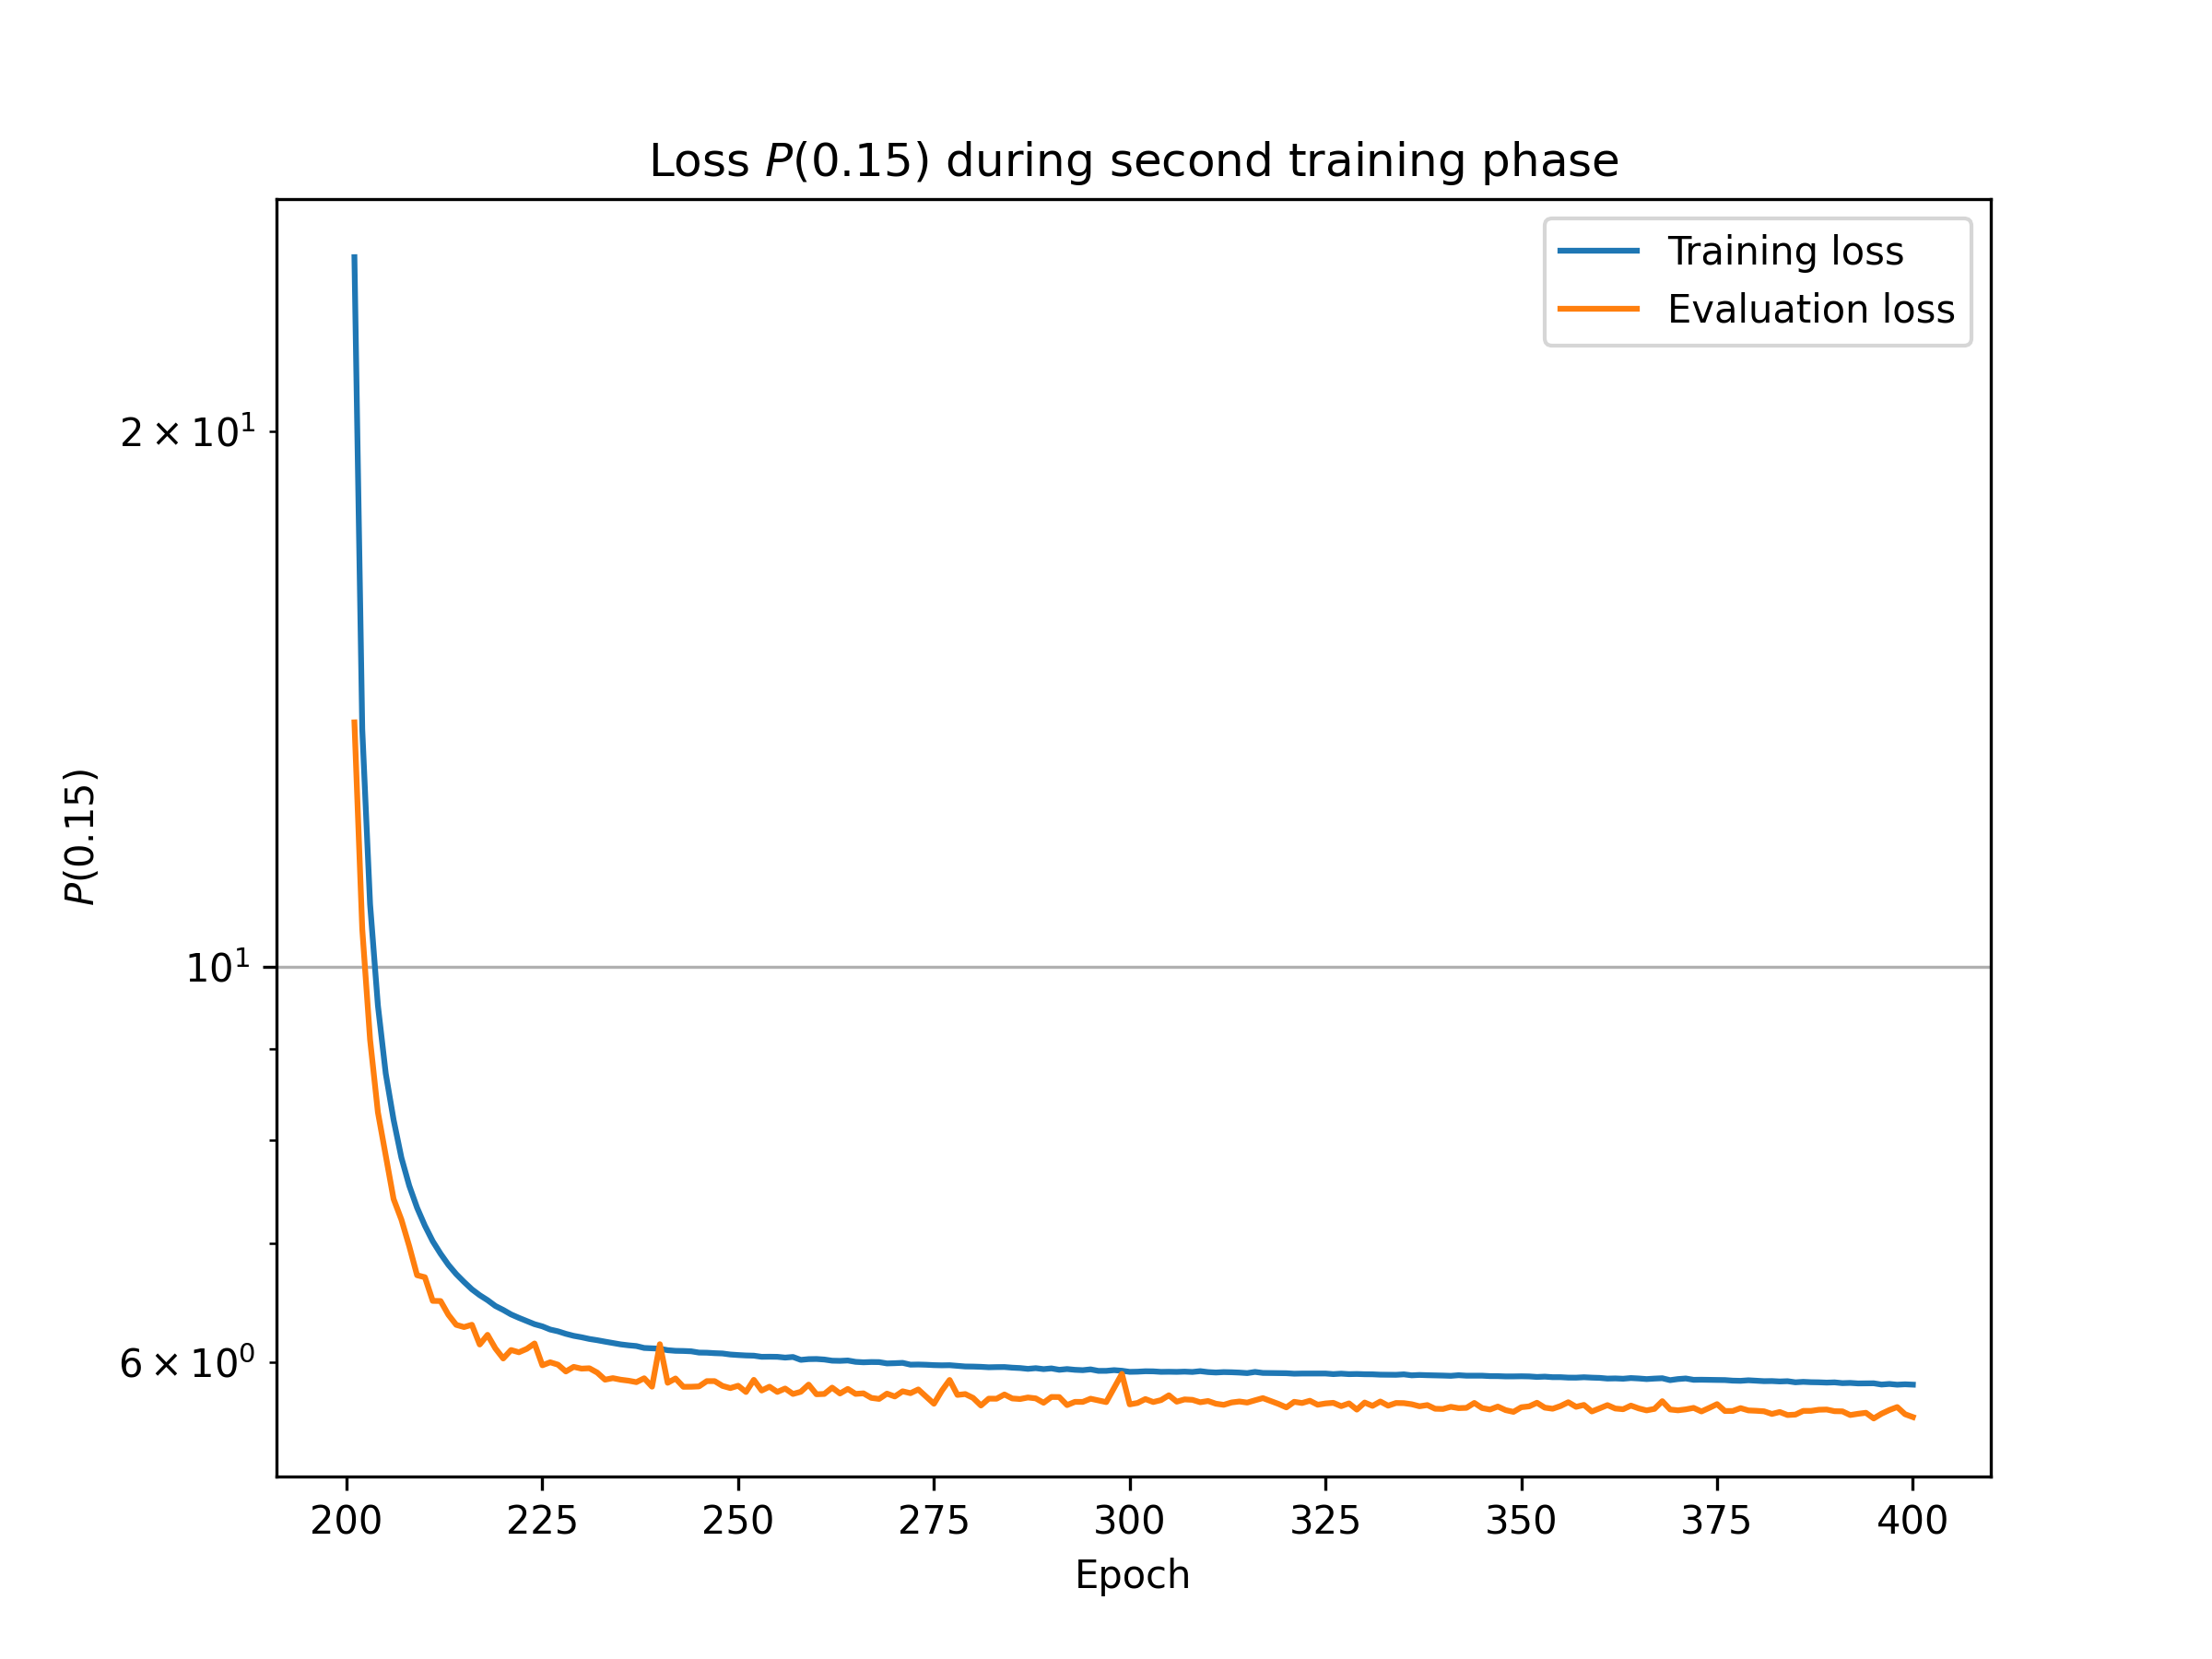
\includegraphics[width=\linewidth]{images/janne/training/phase_2_penal.png}
  \end{subfigure}
  \caption{Profile of the loss $60 \cdot {\cal L}_{reg}$ and $0.25 \cdot P(0.15)$ during the second phase of training}
  \label{fig:janne:phase_2_2}
\end{figure}

\begin{figure}
  \centering
  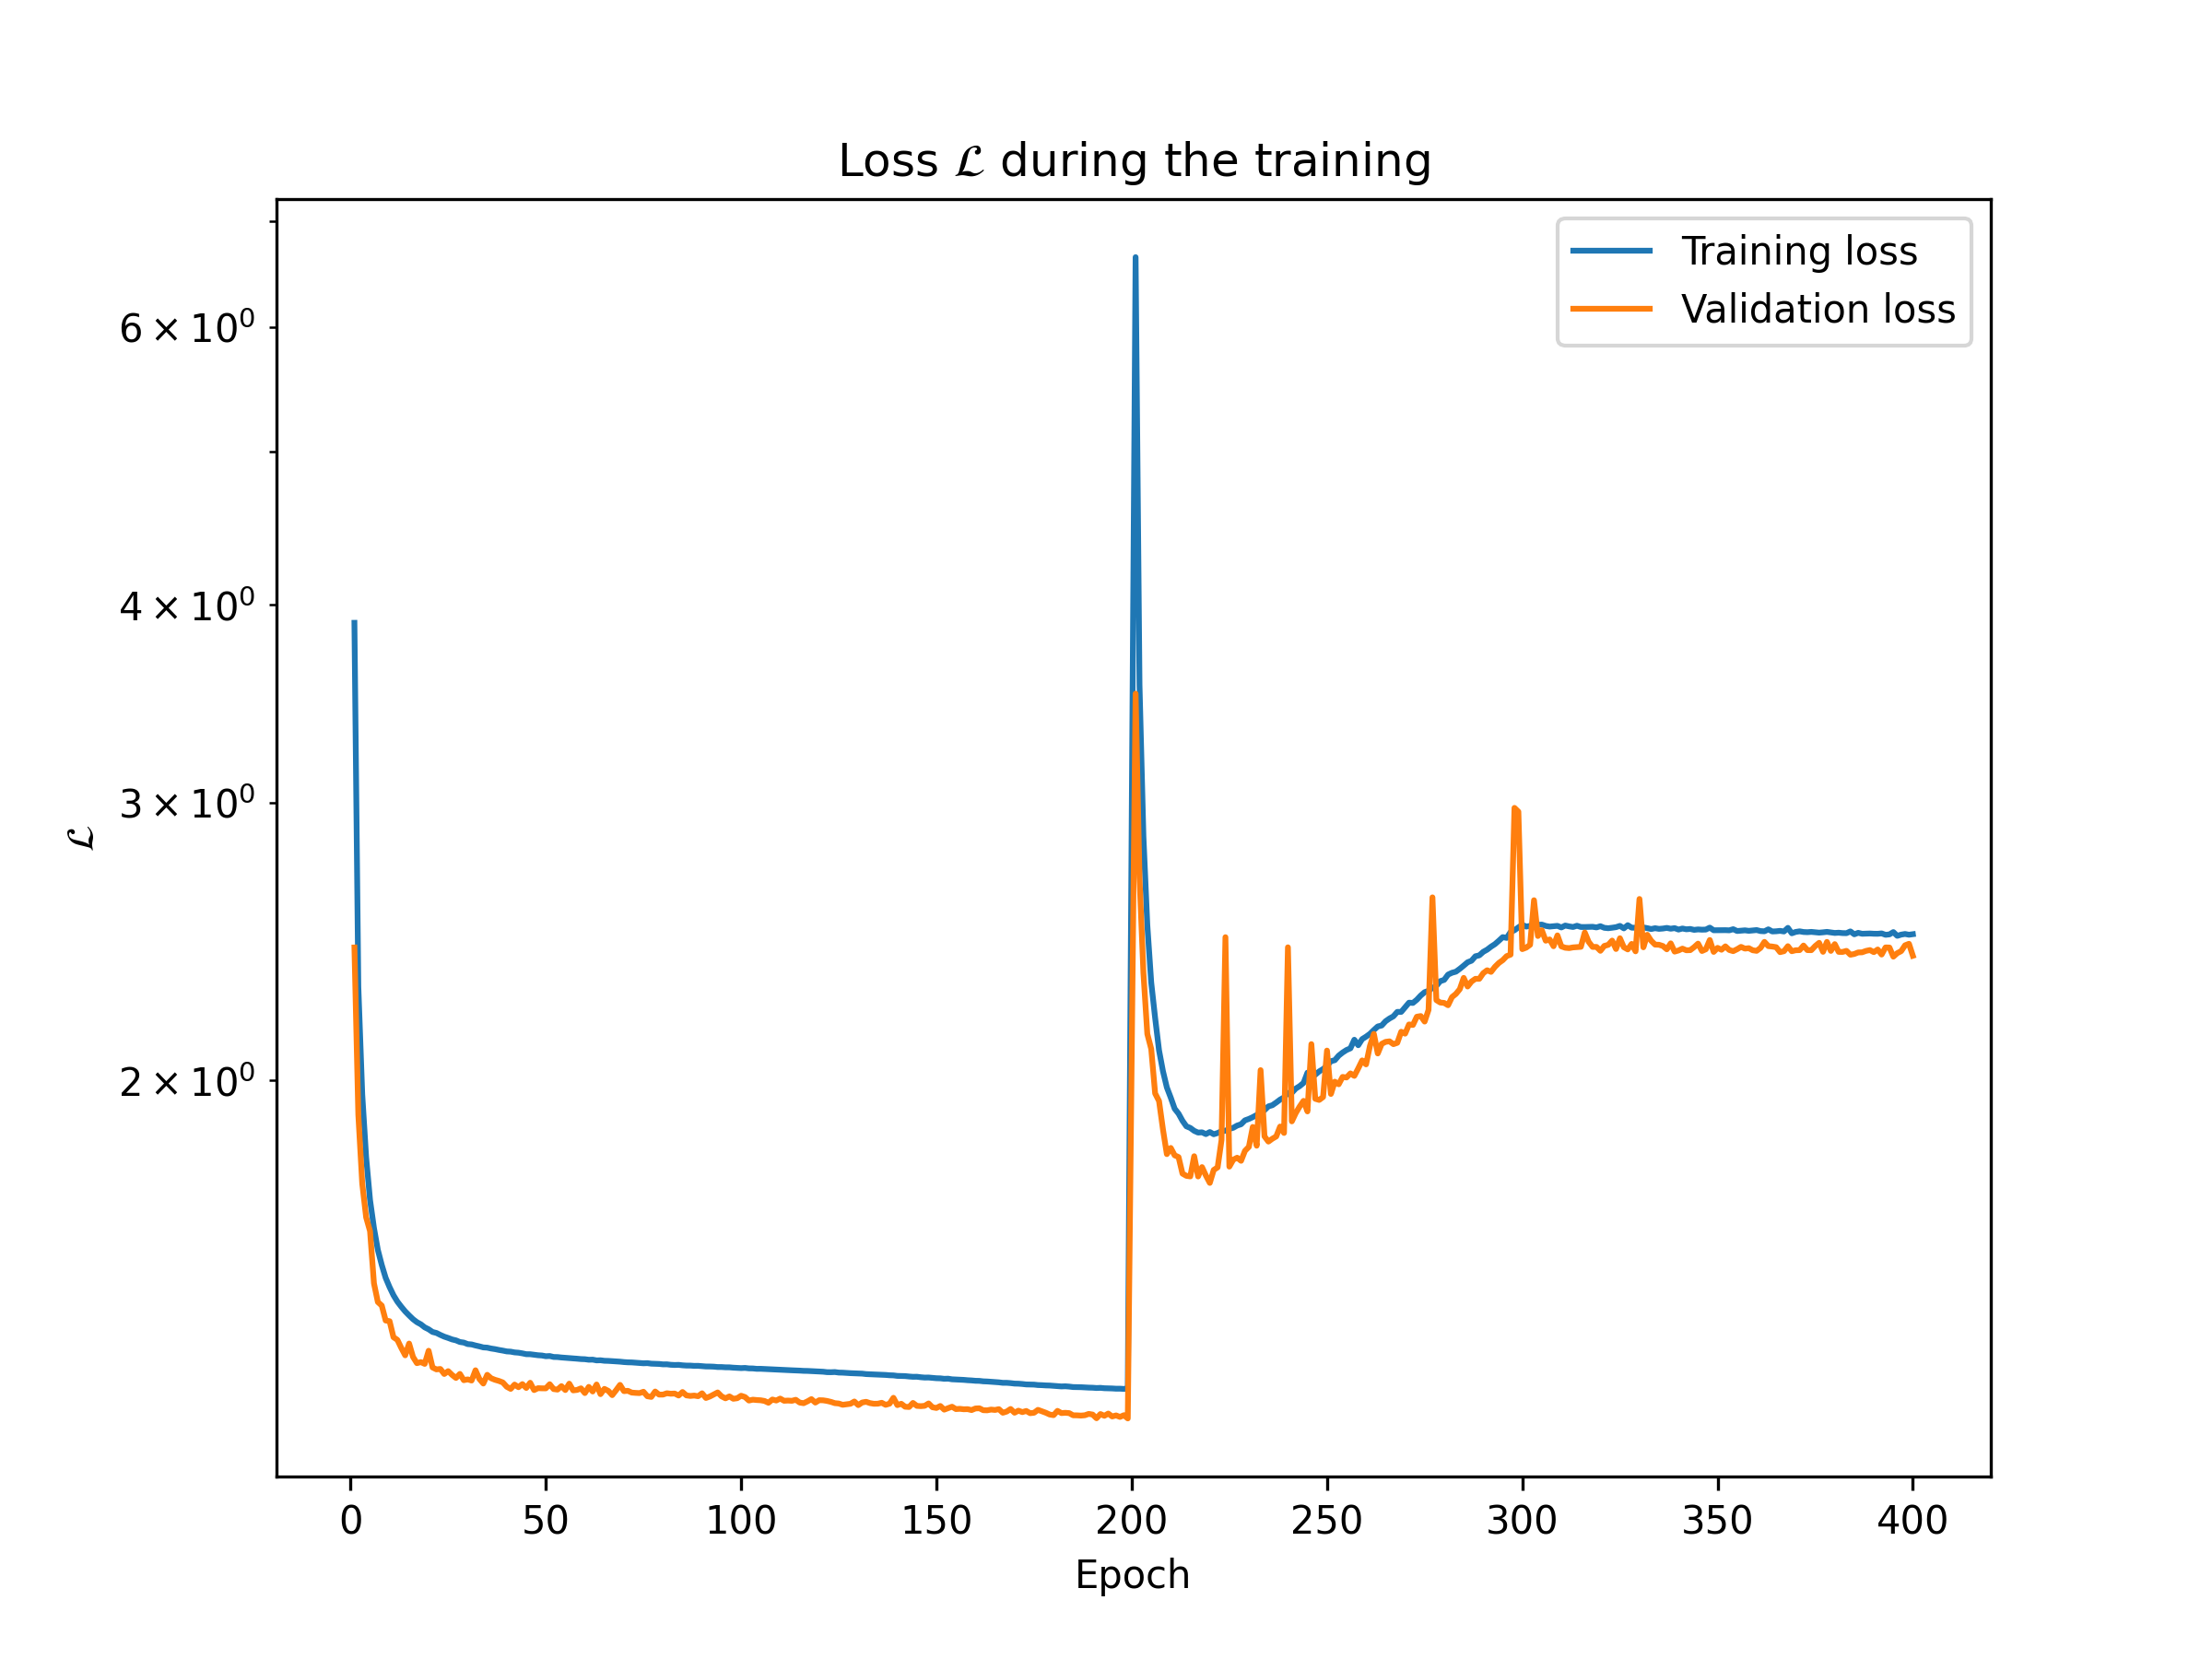
\includegraphics[height=6cm]{images/janne/training/phase_all_l.png}
  \caption{Profile of the loss over the entirety of the training (Phase 1 and 2)}
  \label{fig:janne:phase_all}
\end{figure}

We see in Figure \ref{fig:janne:phase_all} that the loss immediately grows at the start of Phase 2. Obviously, part of this effect is due to the term ${\cal L}_{adv}$ as it tries to perturb the reconstruction but, interestingly, the term ${\cal L}_{reg}$ that ensures the reconstruction of the control sample is still correct continues to decrease over Phase 2. It indicates that, while the penalty term $P(0.01)$ in Phase 1 did some work in reproducing the input event, it was still not enough for the reconstruction to be at the same level as without the ANN.

At the beginning of Phase 2, ${\cal L}_{adv}$ is not equal to one due to the problem mentioned above, but as ${\cal L}_{reg}$ decrease, ``correcting'' the reconstruction, ${\cal L}_{adv}$ grows close to 1. We see that after about 100 epochs of stability in ${\cal L}_{adv}$, the correlation drops a bit from $\sim$ 0.9985 to $\sim$ 0.9975 while ${\cal L}_{reg}$ continues to decrease, hinting at possible room for perturbation.

After 200 epochs of Phase 2, the correlation in ${\cal L}_{adv}$ is still at 0.998, the penalty term $P(0.01)$ is stable and the regularisation loss ${\cal}_{reg}$ is close to stability.

For illustration, events produced by the ANN after 400 epochs are displayed in Figures \ref{fig:janne:hr_he_400} and \ref{fig:janne:lr_le_400}. These are the same event as displayed in Figures \ref{fig:janne:hr_he_200} and \ref{fig:janne:lr_le_200}.

\begin{figure}[ht]
  \centering
  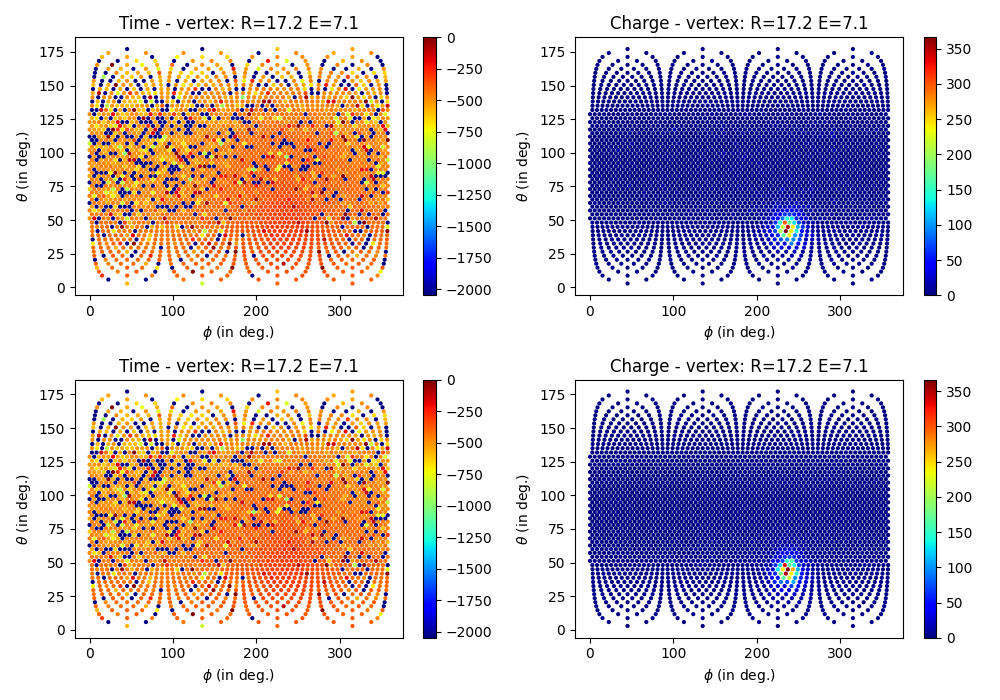
\includegraphics[height=8cm]{images/janne/events/hr_he_400.png}
  \caption{Time channel (on the left) and charge channel (on the right) of a \textbf{radial, high energy event} ($R$ = 17.2 m, $E_{dep}$ = 7.1 MeV), \textbf{Top:} before the ANN perturbation, \textbf{Bottom:} after the ANN perturbation. The ANN have been trained for 400 epochs, just after Phase 2. Time channel in ns and charge channel in $N_{pe}$.}
  \label{fig:janne:hr_he_400}
\end{figure}

\begin{figure}[ht]
  \centering
  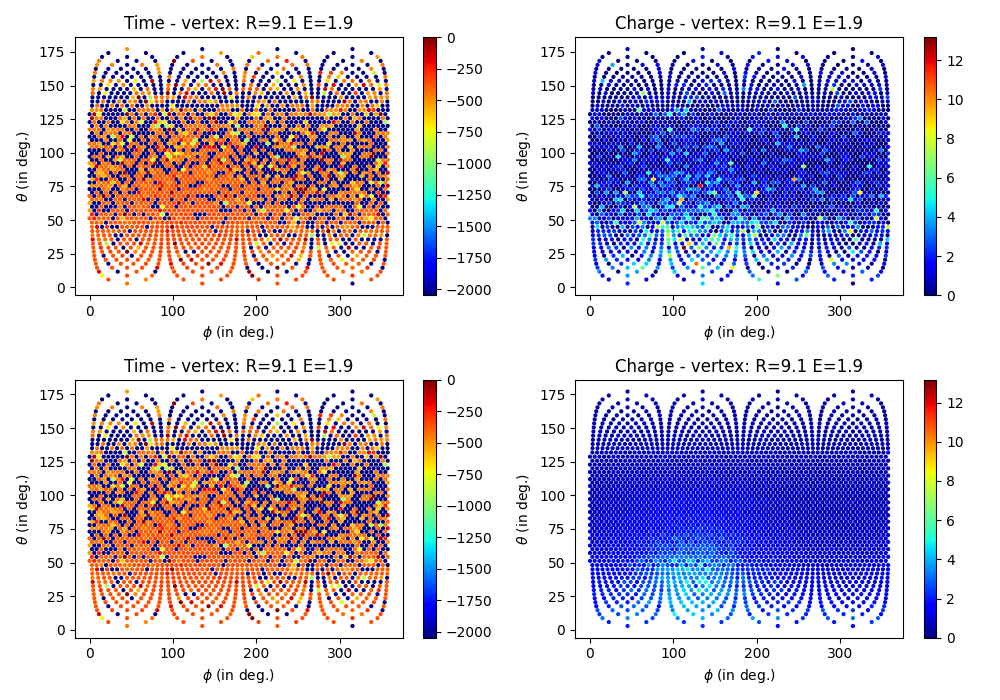
\includegraphics[height=8cm]{images/janne/events/lr_le_400.png}
  \caption{Time channel (on the left) and charge channel (on the right) of a \textbf{central, low energy event} ($R$ = 9.1 m, $E_{dep}$ = 1.9 MeV), \textbf{Top:} before the ANN perturbation, \textbf{Bottom:} after the ANN perturbation. The ANN have been trained for 400 epochs, just after Phase 2. Time channel in ns and charge channel in $N_{pe}$.}
  \label{fig:janne:lr_le_400}
\end{figure}

The same observations that were made after phase 1 still apply after phase 2. The ANN still spreads the charge over multiple pixels for central events, Figure \ref{fig:janne:lr_le_400}, while for radial events it is able to reproduce the small localization of the event.

When looking at the distribution of ratio between the reconstructed energy distribution before and after the application of the ANN, Figure \ref{fig:janne:f_circ_over_f_400}, we observe this time a deficit of events in the high energy bin. This deficit is explained by the comparison between the distribution of relative reconstruction errors, Figure \ref{fig:janne:rec_err_400}, in which we see a small negative bias. This same figure shows a wider loss in resolution when the ANN is present. This is the ANN working to degrade the resolution of the FFNN.

\begin{figure}[ht]
  \centering
  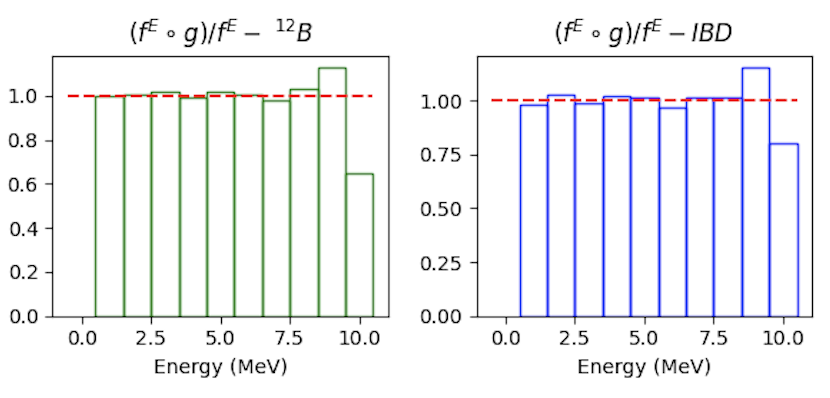
\includegraphics[height=4cm]{images/janne/f_circ_over_f_400.png}
  \caption{Ratio of the reconstructed energy spectra between $({\cal F} \circ {\cal G})$ and ${\cal F}$ at then end of Phase 2 of the training. \textbf{On the left :} For the $^{12}$B dataset. \textbf{On the right :} For the IBD dataset}
  \label{fig:janne:f_circ_over_f_400}
\end{figure}

\begin{figure}[ht]
  \centering
  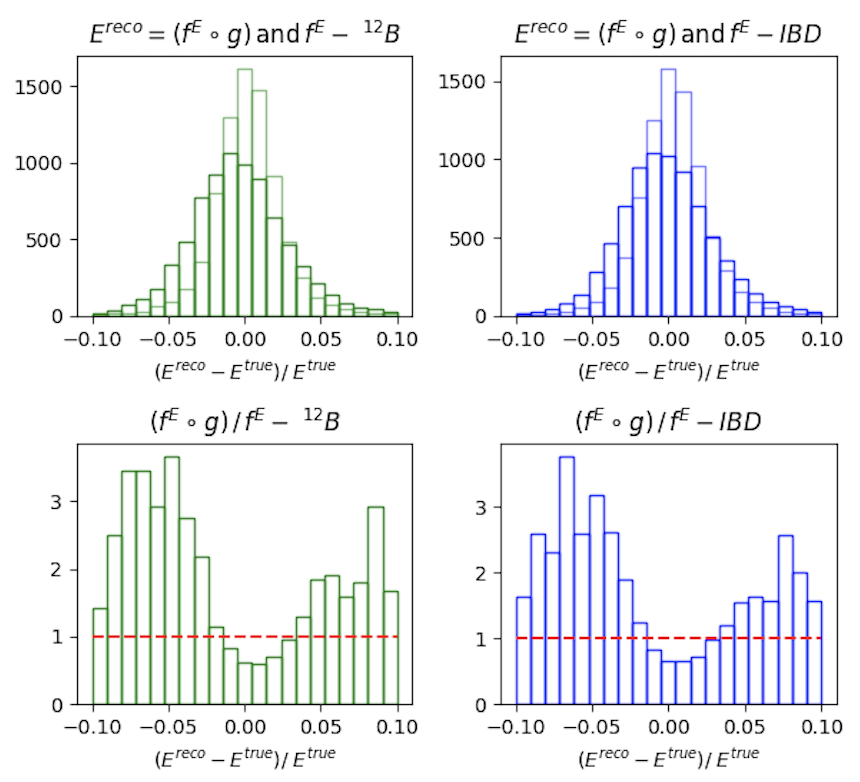
\includegraphics[height=8cm]{images/janne/rec_err_400.png}
  \caption{\textbf{On the top :} Distribution of the relative energy reconstruction error between ${\cal F}$ (light histogram) and $({\cal F} \circ {\cal G})$ (dark histogram) at then end of Phase 2 of the training. \textbf{On the bottom :} Ratio between the light and dark histogram of the top figure.}
  \label{fig:janne:rec_err_400}
\end{figure}

\begin{figure}[ht]
  \centering
  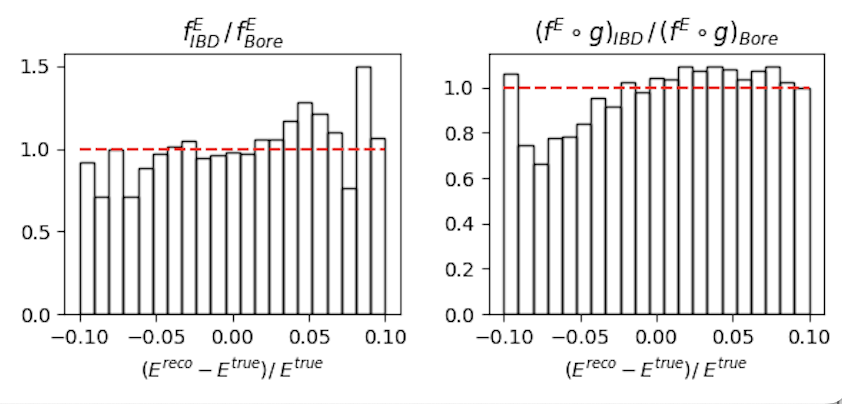
\includegraphics[height=4cm]{images/janne/ann_effect_400.png}
  \caption{Ratio between the relative error on the reconstructed energy between the IBD and the $^{12}$B dataset. \textbf{On the right :} without the ANN. \textbf{On the left :} with the ANN.}
  \label{fig:janne:ann_effect_400}
\end{figure}

Figure \ref{fig:janne:ann_effect_400} shows the ratio between the relative error on the reconstructed energy between the IBD and the $^{12}$B dataset with and without the ANN. We don't see any indicative difference, the ANN even seems to have harmonized the reconstruction error between the two datasets. The ANN is not capable of introducing perturbation that would target only the IBD dataset, it not capable of distinguishing the physics dataset from the control dataset.

This leads us to one of two conclusions. Either this reconstruction algorithm is robust to ANN attacks, or the ANN is not powerful enough to find meaningful attack. We lean to the second proposition. The simple architecture of the ANN, the fact that it does not precisely reproduce events after Phase 1 of the training and the trouble we experienced to balance the loss between ${\cal L}_{adv}$ and ${\cal L}_{rec}$ are clues indicating we can probably produce a more powerful ANN.

\section{Conclusion and prospect}
\label{sec:janne:conclusion}
%\begin{itemize}
%  \item Not enough
%  \item Probably guide the ANN
%\end{itemize}


Reliability and knowledge of our reconstruction algorithms are crucial for the successful conduct of the experiment. The first step to testing and comparing the reconstruction algorithms is to have them publicly available. To this end, I have implemented a BDT for energy reconstruction in JUNO's common software and compared its performance and behavior in detail to the classic likelihood algorithm OMILREC. The strong correlation between their errors indicates that close to no improvement can be made by combining the two algorithms, as they use the same information.

In this chapter, we explore the relevance of using an ANN to produce physically sound perturbations that would distort the reconstructed energy spectrum while being invisible to the control sample. We present a simple architecture. I show the complexity of developing such an architecture; the gradient back-propagation technique poses a number of problems, namely the impossibility of backpropagating through complex and external algorithms.

We have developed a simple reconstruction method to run the ANN against. The current ANN architecture has trouble reproducing precisely the event, even before being tasked to introduce perturbations, and once it tries, it is not able to find such perturbations.

Multiple things can be implemented to explore further with the ANN. As discussed, the ANN has trouble reproducing events; it is possible that the loss ${\cal L}_1 = P(0.01)$ is not sufficient for this task, but also that the architecture is not adapted to our problem. ResNet architectures \cite{he_deep_2016} have already proven that the introduction of residual operations helps the network reach better performance. We can imagine a network where instead of $X' = {\cal G}(X)$ we have $X' = {\cal G}(X) + X$, where the ANN ${\cal G}$ computes only the perturbation instead of a whole new event.

Further work on the loss is necessary. The equilibrium between ${\cal L}_{adv}$ and ${\cal L}_{reg}$ is crucial and should be further studied. A good way to study its effect would be to compare the performance of the ANN for a different set of weights. If one can determine an equilibrium rule between the two, it can be adjusted dynamically during the training, resulting in finer optimisation.

The architecture of the ANN is, for now, very simple; it’s a Fully Connected Deep NN with a bottleneck architecture. Previous work in developing ML for reconstruction \cite{qian_vertex_2021} and the algorithms presented in Chapters \ref{sec:jcnn} and \ref{sec:jgnn} show the relevance of convolutions in the reconstruction, and the work of Gavrikov et al. \cite{gavrikov_energy_2022} presented at the beginning of this chapter hints at the importance of the time and charge distribution. A more complex and refined architecture can probably be more effective.

Another way to improve the ANN would be to find potential discrepancies between the IBD and the $^{12}$B datasets and ``guide'' it to produce those perturbations.

Finally, to use this method on every reconstruction algorithm, we must move away from the back-propagation method, for reasons detailed in Section \ref{sec:janne:back_prop}, and use different methods such as Reinforcement Learning.

\end{document}
